\documentclass{article}
\usepackage[utf8]{inputenc}
\usepackage[english]{babel}
\usepackage{graphicx, color}
\usepackage[a4paper,margin=2cm]{geometry}
\usepackage{hyperref}
\usepackage[numbers]{natbib}
\usepackage{subfiles}
% \usepackage{refcheck}
\usepackage{csquotes}
\usepackage{titlesec}
\usepackage{textcomp}  % \textquotesingle
% \usepackage{fontspec}
% \setmainfont{Symbola}
\usepackage{siunitx}
\sisetup{output-exponent-marker=\ensuremath{\mathrm{e}}}
% \usepackage{dirtytalk}
\usepackage{epigraph}
\usepackage{amsfonts}

% \setcounter{secnumdepth}{4}

\titleformat{\paragraph}
{\normalfont\normalsize\bfseries}{\theparagraph}{1em}{}
\titlespacing*{\paragraph}
{0pt}{3.25ex plus 1ex minus .2ex}{1.5ex plus .2ex}

\begin{document}

\subfile{title-page-ai.tex}

\tableofcontents

\pagebreak

\begin{abstract}
    TODO: abstract

    % https://twitter.com/tscholak/status/1279061409570213895?s=21
    % synthesis is fun but probably not so much without unit tests or types.

    % For reproducibility, we release our code publicly.
\end{abstract}

\section{Research Direction} % \label{sec:research-direction}

\subsection{Program Synthesis}

\epigraph{
    Truly solving program synthesis is the last programming problem mankind will have to solve.
}{
    \textit{\citet{nps}}
}

After chess engine \emph{Deep Blue} defeated grandmaster Kasparov in 1997~\citep{deepblue},
in a freestyle chess tournament in 2005,
both a supercomputer and a grandmaster with a laptop lost to two amateurs using three laptops~\citep{kasparov},
demonstrating the importance of man-machine cooperation.

\begin{displayquote}
    If artificial intelligence (AI) is software 2.0~\citep{software20},
    then \emph{program synthesis} is software 2.0 applied to the field of software development itself.
\end{displayquote}
% I think only few will feel offended by the implication all program synthesis uses AI.

TODO: talk more about the gaps between 1.0/engineering vs 2.0/AI, and how the present work aims to bridge those.

% synthesis
\emph{Program synthesis}~\citep{church1957applications} is the task of automatically constructing a program%
% ~\footnote{
%     While the definition of a program might be debatable as well,
%     and there has been work on predicting type signatures from function names~\citep{wang2018predicting},
%     for the purpose of our paper we will focus on traditional executable programs,
%     rather than e.g. `programs' describing types.
% }
that satisfies a given high-level specification,
be it a formal specification, a natural language description,
full program \emph{traces}, input-output examples,
or an existing program.~\citep{gulwani2017program}.

This enables us to distill our modeled program
to a simplified discrete form that may well be intelligible to humans as well as computers,
opening up opportunities for human-machine cooperation in writing software.
Specifically, this will allow machines to improve on programs written by humans, and the other way around.
As such, program synthesis may bring \emph{hybrid intelligence}~\citep{sun1994computational} to the field of software development.

And in fact, we may already see this in the proliferation of intelligent code completion tools%
~\footnote{
    These include Microsoft's \emph{Intellisense},
    Google's \emph{ML Complete},
    Jetbrains's code completion in their IntelliJ IDE,
    as well as Codota's \emph{TabNine}.
},
as well as in a novel development paradigm in functional programming based on typed holes called \emph{type-driven development}~\citep{brady2017type}.

\subsection{Related fields}

To give more context on how program synthesis fits into the bigger picture,
we will briefly compare it to some other fields: program induction, supervised learning, as well as constraint satisfaction and discrete optimization.

\subsubsection{Program Induction}

Unfortunately the field suffers from competing definitions, blurring the distinction between what constitutes program \emph{synthesis} versus what constitutes program \emph{induction}. In short though, those in either field claim to be more general than the other branch.

The field of \emph{inductive programming}~\citep{popplestone1969experiment,plotkin1970note,fogel1966intelligent}, primarily known for its sub-branch \emph{inductive logic programming}~\citep{muggleton1991inductive} focused on propositional logic, is simply automatic synthesis of inductive logic, and was coined to distinguish itself from the \emph{deductive} techniques used in \citet{church1957applications}'s synthesis of circuits. Under this definition, the term program synthesis is used to refer to its original scope of program generation using deductive techniques.

Whereas in the original problem definition the desired behavior was fully specified, program \emph{induction} aimed to generalize the problem to also tackle automatic generation of programs for which the desired behavior had only partially been made explicit, through e.g. input/output examples or incomplete data.

Under this definition, there is no significant distinction between our present work and program induction's sub-branch of \emph{inductive functional programming}, focused on the generation of programs in functional programming languages such as Lisp~\citep{lisp} or Haskell.

Nevertheless, in current parlance \emph{program synthesis} is often used in a broader scope, extending from the original deductive approach to include inductive approaches as well.
In this view, the two fields are distinguished in that program \emph{synthesis} is defined as to explicitly return a program,
whereas program \emph{induction} learns to \emph{mimic} it rather than explicitly return it.%
~\citep{devlin2017robustfill,gulwani2017program,nps}
While this usage appears to clash with the term program induction as used in inductive \emph{functional} programming,
this view of program induction being limited to this smaller scope likely stems from widespread use of the term in the field of inductive \emph{logic} programming.

This terminology itself is not of much concern for our present paper, as the boundaries between the fields have often been muddy.
Moreover, recent applications of AI to this field have led to the more recent term of \emph{neural program synthesis}~\citep{nps}. Therefore, we will simply settle for using `program synthesis' to refer to the field in general as well.

\subsubsection{Supervised Learning}

The above definition of program synthesis as explicitly returning a program,
% particularly in its \emph{programming by example} (PBE) variant of learning from input-output examples,
is helpful to explain how it differs from \emph{supervised learning},
the machine learning task of learning a function that maps an input to an output based on example input-output pairs~\citep{russell2002artificial}.

Deep neural learning methods may be applied to any branch of program synthesis,
and several of these may in fact be tackled using setups involving supervised learning.
Of particular note here however is a branch referred to as \emph{programming by example} (PBE),
which like supervised learning is based on the question of how to reconstruct a mapping between input and output --- in the supervised learning context also referred to as \emph{features} and \emph{labels}, respectively.

What sets these apart is that,
whereas supervised learning would construct such a model in a continuous vector space,
allowing probabilistic interpretations of the data to be taken at prediction time,
% [(X,Y)] -> X -> IO Y
PBE instead fits its model into the discrete form of a given \emph{grammar} to produce a program,
forcing one to instantiate such a model from probabilistic data interpretations.
% [(X,Y)] -> IO (X -> Y)

This also explains the relative benefits of these two fields:
supervised learning may stay in the continuous realm,
characterized by differentiable models optimizable by backpropagation~\citep{backproprnn},
and not limited in expressivity by the limitations of any particular grammar or set of operations.
This makes it well-positioned to solve problems deemed too complex for traditional programming, such as image recognition.

Program synthesis techniques may instead construct a traditional program,
which may be deterministic, can generalize better~\citep{nps}, and be provably correct~\citep{nps},
as well as potentially faster to execute than predictions using the equivalent supervised learning model.

Moreover, using programs as a common denominator between human and machine-based programmers makes for human-intelligible machine-made models,
relevant in the field of \emph{interpretable} or \emph{explainable artificial intelligence}
~\footnote{
    One may note that if the goal in using program synthesis is to make models more interpretable,
    one could potentially start out by training a neural model,
    then approximate this by synthesizing a program similar to it.
    And in fact, \citet{pirl} apply exactly this approach for reinforcement learning.
},
while also enabling human-machine cooperation in the production and maintenance of software.

Furthermore, program synthesis may help tackle the problem in AI of \emph{composability}:
programs in their essence \emph{compose} operations into larger logical building blocks,
to be reused or further generalized.
In supervised learning, on the other hand,
one would traditionally need to retrain the model in the event a new predictor class is added,
which depending on the model complexity may be quite costly.%
~\footnote{
    While the effort of retraining may be alleviated using \emph{pre-training} to only retrain the later layers,
    this issue of retraining still persists.
}
This challenge of composability in AI has also been studied by the field of \emph{hierarchical reinforcement learning}~\citep{hierarchicalrl}.

In program synthesis, one may take an existing program, and synthesize variants intended to generalize the existing logic to match the new data.~\citep{myth}
This makes program synthesis well-suited to facilitate the automation of programming.%
~\footnote{
    One may note that this would technically enable the synthesis of programs implementing machine learning models as well.
    However, such an approach would make for a relatively expensive evaluation function,
    and as such is traditionally left to the field of \emph{neural architecture search}.
}

In other words, whereas supervised learning makes for simpler learning,
as it foregoes the need to define a synthesis grammar and operator set,
program synthesis may make for programs that are potentially more efficient,
composable,
and providing better interaction with humans.

This last point is both in terms of being understandable,
which for the machine learning models produced in supervised learning requires adding the non-trivial field of \emph{explainable AI}~\citep{gunning2017explainable},
while program synthesis also allows more easily incorporating knowledge of human experts,
by allowing them to offer relevant operators.
% table of relative merits: supervised learning side, pros: able to model ill-defined logic, more suited for stochastic predictions

\subsubsection{Constraint satisfaction vs. discrete optimization}

% relation to https://en.wikipedia.org/wiki/Constraint_programming : that seems a subset associated with logic programming
% relation to SMT: that's first-order logic, synthesis is second-order
% relation to SAT: that's SMT without linear constraints, so even less expressive
While its definition may appear to frame program synthesis as a type of \emph{constraint satisfaction} problem (CSP),
where a program either does or does not satisfy the given specification,
% ~\footnote{https://en.wikipedia.org/wiki/Constraint_satisfaction_problem}
one could also opt to approach it as a \emph{discrete optimization} problem,
% relation to https://en.wikipedia.org/wiki/Combinatorial_optimization : that one assumes a finite set of objects? 
as specifications such as input-output examples allow us to count the examples our candidate program satisfies.

Intuitively, a program satisfying part of our examples may be regarded as closer to a solution than one that does not satisfy as many.
Furthermore, additional considerations such as performance may further push us to find a solution that not only calculates outputs correctly but also runs within reasonable time or memory constraints.
These then provide a quantifiable feedback measure for us to optimize.

However, constraint satisfaction and discrete optimization were intended to solve fully specified problems (\emph{deduction}),
while in modern-day program synthesis, as we will explain later,
we usually need to settle for a \emph{partial} specification of the intended program's behavior (\emph{induction}).

In other words, in such an inductive setting one cannot even definitively tell whether one program is better or worse than another on unspecified \emph{intended} behavior,
meaning the metric that would be used for constraint satisfaction or optimization may not be representative of the actual problem.
This is a general difference between constraint satisfaction and optimization versus pattern recognition techniques including machine learning:
in the latter case, the actual goal is to \emph{generalize} learned behavior to an unseen test set,
rather than merely performing well on known examples.

As such, applying such techniques to the field of program synthesis using partial specifications may lead us to the problem of \emph{overfitting}:
while found solutions might well satisfy the \emph{specified} behavior,
the question would be whether these would also \emph{generalize} to match our \emph{intended} behavior,
as is the goal in PBE.

\subsection{Challenges}

\subsubsection{Challenge of program synthesis}
% \subsubsection{Challenge of programming by example}

While considered a holy grail of computer science~\citep{gulwani2017program},
program synthesis in general is a challenging task, characterized by large search spaces,
e.g. a search space of $10^{5943}$ programs to discover an expert implementation of the MD5 hash function.~\cite{gulwani2017program}

\subsubsection{Challenges of type-theoretic programming by example} \label{sec:typepbe}

One issue with type-theoretic approaches to PBE, later introduced in further detail,
is that while such search methods are able to make use of both input/output examples and types in their search,
there is no sense of learning across problem instances to further reduce synthesis time.

\subsubsection{Challenges of neural programming by example} % \label{sec:challengesnps}

For neural methods in PBE, the original challenge of large search spaces means
it will not be viable to proportionally scale our training sets by program size.

Furthermore, whereas a program synthesizer may be programmed or taught to output programs adhering to a given grammar,
we may generally only be able to evaluate the quality of \emph{complete} programs:
there is typically no guarantee that \emph{partial} constructions of the program would \emph{also} qualify as a full executable program adherent to the grammar.
As a result, neural synthesizers will have little intermediary feedback to go by, limiting their effectiveness.

But if only \emph{complete} programs can be evaluated for validity and behavior, then 
we will be ill-equipped to provide synthesizers with an accurate understanding of partial programs,
which make up for a large part of our prediction steps.
As such, it would be desirable to somehow supervise the intermediate prediction steps.
This echoes \citet{nps}'s conclusion that one area of research in neural program synthesis that requires further exploration is
\emph{specifically designing neural architectures} to excel at the difficult problems of program synthesis.

% \paragraph{Challenges of sequential-based neural programming by example}

Most neural synthesis techniques, particular those using a \emph{sequence-to-sequence} approach,
additionally face the issue of dissonance between their representation of complete programs and that of intermediate states.%
~\footnote{
    While in tree-based synthesis techniques it might not be possible to \emph{execute} partial programs either,
    this should at least result in an (incomplete) \emph{abstract syntax tree} (AST),
    which should be significantly easier to learn to embed given the knowledge of how to embed a complete AST than it would be to embed a program that does not even parse.
}
As such intermediate states do not in general constitute valid programs,
these neural synthesizers have an additional task to solve:
compensating for their lack of an inherently meaningful incremental state.

\subsection{Research question}

\subsubsection{Complementary strengths}

Our key observation here is thus that input-output examples and types are quite complementary as specifications constraining our program behavior.
Input-output examples are relatively expressive, but may only help us to evaluate the quality of complete programs.
Types, on the other hand, are by themselves not usually descriptive enough of our task,
but may help us to evaluate and inform further incremental synthesis steps even of incomplete programs still containing \emph{holes},
i.e. placeholder nodes in the AST to be filled by the synthesizer.

\subsubsection{Hypotheses}

We therefore hypothesize that program synthesizers may thus capitalize on this synergy by utilizing both types of information,
rather than settling for only one of the two, as most existing methods have done.%
~\footnote{
    While one might wonder if this constrains our idea to the subset of PBE problems where type information is available,
    this limitation is essentially meaningless:
    when one has input-output examples in a programming language supporting type inference,
    one would already have the types of these input-output examples.
    This would render our idea applicable for practically any (neural) methods for PBE.
}%
~\footnote{
    Whereas one might wonder if a focus on types may constrain our method to synthesizing statically typed languages,
    in the functional paradigm in particular, we believe there are workarounds to this.
    While we certainly believe users may find switching to a statically typed functional language to be beneficial~\citep{hughes1989functional},
    an alternative would be to (1) have one algorithm translate the partial program to a statically typed language,
    (2) complete the program using program synthesis from there,
    then finally, (3) using a third algorithm, translate the full program back to the target language.
}

Specifically, we hypothesize that the effectiveness of neural program synthesis may be improved by
adding type information as additional features during training and testing,
which in \emph{abstract syntax tree} (AST) based neural program synthesis may help supervise each incremental prediction step.

\begin{displayquote} % \label{hyp:types}
    \emph{Research question \#1: can neural program synthesis methods benefit from using types as additional features?}
\end{displayquote}

An alternative approach would be to enumerate any possible options for a given node,
then filtering this list of options based on such compiler feedback.%
% ~\footnote{One potential concern here is the scalability of such enumeration as the number of valid options grows.}

This is indeed done for type-based program synthesis~\citep{myth},
and we hypothesize neural synthesis approaches may benefit from such pre-filtering as well,
reducing synthesis to a ranking problem of (partial) candidate programs.

\begin{displayquote} \label{hyp:filter}
    \emph{Research question \#2: can neural program synthesis methods benefit from type-based filters?
    %  by reframing the problem to learning-to-rank?
    }
\end{displayquote}

% \pagebreak

\section{Expected Contribution} % \label{sec:expected-contribution}

The present work aims to be the first experiment to:
\begin{itemize}
    \item bring the \emph{type-based information} traditionally used in functional program synthesis into the newer branch of neural program synthesis,
    % \item \emph{bridge} the two fields, such as to find a best-of-both-worlds golden mean;
    better \emph{constraining the search space} to improve the effectiveness of neural program synthesis methods;
    \item show that the neural synthesis of statically typable programs may benefit from techniques \emph{specific} to this domain, and therefore for the purpose of automatic programming merits further study in itself;
    \item offer an \emph{open-source implementation} of the algorithm described in \citet{nsps};
    \item generate a \emph{dataset} for neural synthesis of functional programs, and lay out how to do this, including an open-source implementation, addressing the current reliance on hand-crafted curricula~\citep{nps};
    % provide an implementation that may be one of the first machine learning projects utilizing
    % \item showcase \emph{static tensor typing} as offered by the \emph{HaskTorch} deep learning library~\citep{hasktorch}.
\end{itemize}

% \pagebreak

\section{Literature review} \label{sec:litreview}

To provide some background to our hypotheses,
we will use this section to first give a brief overview of how programming by example (PBE) fits into the broader picture of program synthesis,
as well as what existing approaches there have been to PBE,
including the \emph{neuro-symbolic program synthesis} model we build upon ourselves.

On types of synthesizers,
\citet{gulwani2017program} introduce a taxonomy based on three key dimensions:
\begin{itemize}
    \item the kind of \emph{constraints} that it accepts as expression of \emph{user intent};
    \item the \emph{space} of programs over which it searches;
    \item the \emph{search technique} it employs, i.e. the synthesizer.
\end{itemize}

While the common thread in program synthesis is that our intended output takes the form of a program,
sub-branches of this field are primarily defined by the types of input we use to come to this output,
i.e. the constraints on expressions of user intent and program search space in the above classification.

We will give a brief overview of such variants of program synthesis in the next section,
with some minor focus on search technique as influenced by the previous criteria.
Search technique we will explore in further depth for PBE in Section \ref{sec:pbe}.

\subsection{Types of program synthesis} \label{sec:synthtypes}

% \subsubsection{Synthesis from formal specifications}

Program synthesis was traditionally studied as a computer science problem,
where the problem was typically framed using a \emph{formal specification}.
This problem was then tackled using e.g. an enumerative search, deductive methods, or constraint-solving techniques.~\citep{gulwani2017program}
However, such formal specifications ended up about as hard to write as the original program,
rendering this approach to the problem not very useful.

Closely related to this field is the idea of synthesizing a program solely from its \emph{type signature}.~\citep{djinn,synquid}
Traditionally types would make for \emph{inductive} synthesis,
i.e. only making for an \emph{incomplete} program specification,
% using types of a level that users may be more familiar with,
% which may include polymorphic types or even algebraic data types,
but this may end up not sufficiently expressive:
while certainly constraining the program space,
input/output examples may still be needed to disambiguate between potential candidate programs.
Adding such examples brings us to the branch of \emph{type-theoretic programming by example},
which we will introduce in further detail in Section \ref{sec:typepbe}.
Program synthesis approaches using types have in fact commonly focused on using functional programming languages as the synthesis language.%
~\citep{synquid,eguchi2018automated,scythe,scout,gissurarson2018suggesting,idris,lenses}

There have also been attempts to get such a type-based approach closer to \emph{deductive} synthesis,
i.e. making for a \emph{complete} behavioral program specification,
through the use of e.g. refinement types~\citep{synquid} or succinct types~\citep{guospeeding}.
However, these approaches tend to fall into a similar pitfall as synthesis from \emph{formal specifications},
requiring the user to write such a detailed type specification that they might have as well just written the program directly.%
~\footnote{
    However, perhaps one might instead also be able to synthesize this detailed type specification,
    % However, perhaps one might instead also be able to approach this as a \emph{hierarchical probabilistic model},
    % first synthesizing this detailed type specification,
    giving the benefit of additional formal guarantees from our actual program that we could then synthesize from this type specification!
}

% % \subsubsection{Synthesis from natural-language descriptions}

% Synthesis from \emph{natural-language} descriptions%
% ~\citep{neuralprogrammer,zhong2017seq2sql,shin2019program,nsm},
% also known as \emph{semantic parsing},
% like PBE
% % is an example of \emph{inductive} synthesis:
% % as we are no longer tied to a formal specification,
% lacks a formal specification,
% as the language used is not necessarily constrained.
% As such, this ends up as a supervised learning problem:
% we take sample natural language inputs,
% and try to learn their corresponding resulting programs.

% This area is closely connected to the field of
% \emph{personal virtual assistants}~\citep{virtualassistant,genie},
% typically combining program synthesis with \emph{speech recognition}%
% ~\citep{juang1991hidden,graves2013speech},
% where response actions may be regarded as constrained synthesized programs,
% although these might also feature unconstrained \emph{dialogue}~\citep{li2016deep} responses,
% as well as \emph{goal-oriented} or \emph{task-oriented dialogue}~\citep{bordes2016goaldialogue,li2016taskdialogue}.
% This task has also been combined with \emph{programming from examples}.~\citep{polosukhin2018neural}

% % \subsubsection{Program repair}

% \emph{Program repair} is a synthesis task where the input to the synthesizer is a (broken) program that is to be fixed by making changes to the program.~\citep{demsky2006inference,kaleeswaran2014minthint}
% This can be used in e.g. IDEs, to suggest users how they might potentially fix syntax errors or misspelled variables in their code.

% As the input to this synthesis branch consists of existing programs,
% it also has quite some overlap with \emph{static code analysis}~\citep{louridas2006static,brockschmidt2018generative},
% which is about gaining insights into snippets of source code,
% and as such may help provide features relevant for use in program repair.

% % \subsubsection{Source-to-source translation} \label{sec:source2source}

% Similar to program repair, \emph{source-to-source translation}%
% ~\citep{loveman1977program,albrecht1980source,partsch1983program,waters1988program,visser2005survey,czarnecki2006feature,chen2018tree,lachaux2020unsupervised}
% is a branch of synthesis where both the input and output are a program.
% However, rather than fixing an existing program,
% the task here is to learn a specific \emph{translation} task,
% e.g. from one programming language to another.
% Over recent years, this field has become an area of application for \emph{neural machine translation}.%
% ~\citep{cho2014nmt,kim2019translating}

% \subsubsection{Programming by Example (PBE)}

Compared to formal specifications, it was found that for users,
input-output examples were a more attractive way to specify desired program behavior,
although as an incomplete specification this made for a harder problem from the perspective of the synthesizer.~\citep{bodik2013algorithmic}
This field is named \emph{programming by example} (PBE).

As the specification is incomplete here, PBE is considered \emph{inductive} synthesis, as opposed to the \emph{deductive} synthesis where we do have a complete specification.
In other words, from the perspective of the synthesizer, PBE is generally a more difficult problem.

PBE may be further split up according to the type of program to be synthesized~\citep{bodik2013algorithmic},
generating \emph{logic programs} (assigning truth values to variables),
or generating \emph{functional programs} (e.g. Lisp, Haskell).
PBE too has branches based on deductive techniques (including \emph{type-theoretic} PBE),
inspired by synthesis from formal specifications.
% Note that these categories are not necessarily mutually exclusive:
% a synthesizer might for example have a natural language input,
% while using this to say generate a functional program.
% Either way,
Our work will focus on PBE in the category of functional programs,
where the goal is to automate traditional programming tasks.

% \subsubsection{Synthesis from traces}

Synthesis from program \emph{traces}~\citep{koskimies1994automatic},
and the related synthesis from \emph{Linear Temporal Logic} (LTL)
specifications~\citep{camacho2019towards}, are about
a system reacting to sequences of inputs to mimic the desired program behavior.
These are useful for e.g. specifying the expected behavior of user interfaces.
Essentially this task may be viewed as a generalized version of PBE,
adding the additional challenge of figuring out which inputs triggered which state changes.

% \subsubsection{Neural program synthesis}

Over recent years, synthesis problems have been explored using \emph{machine learning} approaches,
under the name of \emph{neural program synthesis} (NPS)~\citep{nps}.
This area is about learning to solve a class of synthesis problems given data.
Note that this is a synthesis \emph{technique}, whereas the the above categories are synthesis \emph{problem types}.

Whereas traditional approaches in program synthesis (and particularly PBE) focused on constraining the large discrete search space,
such as deductive and constraint-solving approaches,
\emph{neural} program synthesis instead tends break down the problem by incrementally generating programs,
using continuous representations of the state space to predict the next token.
% be it in a sequential fashion~\citep{npi,neuralmachinetranslation,alphanpi},
% or in a structured one based on ASTs~\citep{nsps}.

\subsection{Existing approaches to programming by example} \label{sec:pbe}

PBE has traditionally known heuristics such as
\emph{Version Space Algebras} (VSAs)~\citep{mitchell1982generalization},
which aim to constrain grammar productions by using
\emph{candidate elimination} to keep track of a \emph{hypothesis space}.

Another useful tool is \emph{ambiguity resolution},
i.e. requesting user input to resolve ambiguity
in the event that multiple candidate programs
fulfill the given input-output example pairs.%
~\citep{gulwani2017program}
While we will come back to ambiguity resolution as it is
alleviated by \emph{active learning}~\citep{settles2009active}, as we discuss in Section \ref{sec:active},
these two techniques are primarily used to complement
other methods we will introduce here now.

Please do note that program synthesis has been somewhat different
from other branches of machine learning, such as image recognition:
although there have been competitions like the
\emph{Syntax-Guided Synthesis competition} (SyGuS-Comp)~\citep{sygus},
unfortunately the field has been so diverse that there has been only limited
standardization of benchmarking tasks to compare approaches,
as \emph{ImageNet}~\citep{deng2009imagenet} had done for computer vision tasks.%
% ~\footnote{
%     First off, neural and search-based methods tend to use different performance metrics,
%     with neural methods typically using accuracy (optionally over a given number of sampled programs),
%     while search-based methods tend to evaluate based on average time to solution on any given task function.

%     Furthermore, some synthesis approaches use additional information next to input/output samples,
%     such as natural-language descriptions~\citep{polosukhin2018neural} or types~\citep{myth}.

%     In addition, many synthesizers attempt to explore different features and techniques,
%     which oftentimes place limitations on the supported \emph{domain-specific languages} (DSLs),
%     and thereby task datasets that can be tested on.

%     Such synthesizer features may include
%     variables, recursion, pattern matching, arbitrary constant values,
%     invertible logic (when depending on this a synthesizer may not support non-invertible operators)~\citep{flashmeta,prose},
%     differentiable languages (which similarly would not support non-differentiable operators)~\citep{forth,terpret,houdini,feser2016differentiable,rocktaschel2017end,abadi2019simple},
%     and parametric return types (our current thesis).

%     Lastly, the use of functional vs. imperative DSLs also affects synthesizers,
%     with the former typically being amenable to type-based approaches (our current thesis),
%     while the more sequential imperative paradigm is typically more supportive of reinforcement learning approaches,
%     where each incrementally added program step may already be executed for immediate learning feedback~\citep{npi,alphanpi}.

%     While ideally, in the future synthesizers of different types should become more fully-featured,
%     in practice, there are various barriers to this:
%     \begin{itemize}
%         \item not all synthesizers aim to tackle complex DSLs
%         (e.g. settling for bytecode-based DSLs for the purpose of \emph{super-optimization}~\citep{schkufza2016stochastic}, i.e. optimizing the performance of an existing program);
%         \item for research purposes fleshing out synthesizer features may also distract from making the minimal case demonstrating a given idea,
%         as other requirements might not be desirable if not needed
%         (e.g. limiting to only invertible or differentiable operators);
%         \item additional requirements may not be mutually compatible or sensible to combine in the first place
%         (e.g. functional DSLs with synthesizers supporting types as additional information vs. synthesizers using reinforcement learning to execute programs step by step for immediate feedback).
%     \end{itemize}
% }

While this means we will not present statistics
comparing the performance of these various approaches,
we will instead lay out their conceptual differences and weaknesses.

\subsubsection{Search-based programming by example}

Under search-based methods for programming by example we will classify any approaches that do not evolve \emph{learning} to synthesize by means of a neural component.

While the approaches in this category range from naive to sophisticated,
they unfortunately share a common drawback:
whereas neural synthesizers allow one to tweak a \emph{loss function} to take into account various sub-goals,
non-neural synthesizers have no sense of \emph{learning}
from existing programs or across problem instances,
meaning they will have trouble achieving:
\begin{itemize}
    \item \emph{generalizability}~\citep{nps};
    \item \emph{interpretability} to humans (human \emph{source code bias}, i.e. make generated code more similar to the way it is written by humans)~\citep{nps};
    \item \emph{synthesized program performance} (as measured in e.g. raw CPU time)~\citep{schkufza2016stochastic};
    \item an increase in \emph{synthesizer performance},
    as they must solve any new synthesis task essentially from scratch,
    and could never have as much information to this end as a neural synthesizer,
    which may in fact be able to use arbitrary learned features~\citep{odena2020learning}.
\end{itemize}

\paragraph{Enumerative search}

The naive approach to synthesis would be to enumerate all the possible programs in our search space,
and for each one evaluate whether it satisfies our task specification.
This is called \emph{enumerative} or \emph{depth-first search} (DFS).
As one might expect, such an approach does not generally scale well with search space size however.

% \paragraph{Evolutionary algorithms}

% \emph{Evolutionary algorithms}~\citep{eiben2003introduction} are a black-box optimization method of potentially discrete functions.

% \emph{Genetic programming} is a branch of evolutionary algorithms based on tree representations,
% rendering it viable to evolve programs using some AST representation.~\citep{koza1994genetic}
% Such evolution is a search method that consists of generating programs similar to existing promising candidates, using either mutations or combinations of existing candidate solutions.

% However, while such heuristics help improve on the baseline of enumerative search,
% optimization is still a one-shot exercise:
% it has little notion of \emph{learning} from previous problems to improve performance on future similar problems.%
% ~\footnote{
%     Technically one way to let an evolutionary algorithm learn would be to seed runs on new problems using solutions from previous similar problems.
%     However, such choices would be left up to the user,
%     and are not something that the evolutionary algorithm itself is able to help out on.
%     In practice, even under the same class of problems,
%     different problem instances will likely require different end solutions,
%     largely rendering this hack moot.
% }
% As such, evolutionary approaches have been more popular in areas where their strategy of \emph{local search} would pose an advantage, such as for \emph{super-optimization}~\citep{schkufza2016stochastic} (optimizing the performance of an existing program) and \emph{program repair}~\citep{weimer2009automatically,forrest2009genetic}.

% \paragraph{Active learning and Bayesian optimization} \label{sec:active}

% % \emph{Active learning}~\citep{settles2009active} and
% % \emph{Bayesian optimization}~\citep{mockus2012bayesian}
% % are two techniques intended to minimize a required number of
% % expensive evaluation rounds in modeling discrete functions.
% % Their difference however lies in their intended objective:
% % the objective in \emph{active learning} is to most accurately
% % model the underlying function, while in
% % \emph{Bayesian optimization} the objective is to maximize

% \emph{Bayesian optimization}~\citep{mockus2012bayesian}
% is a technique used in the modeling of discrete functions
% intended to minimize a required number of
% expensive evaluation rounds while locating a global maximum.

% The objective \emph{Bayesian optimization} is to maximize
% a given reward (as a total over the number of evaluations),
% which renders it a trade-off of \emph{exploration} versus
% \emph{exploitation}~\citep{distillbo} similar to that of reinforcement learning.

% % Within program synthesis, active learning, which here consists of human-computer interaction to improve learning,
% % is primarily used to
% % facilitate effectively requesting interactive user feedback when
% % trying to synthesize a particular function in PBE when faced
% % with ambiguity of user intent.~\citep{shen2019using}%
% % ~\footnote{
% %     Interactive user feedback is a useful technique in the face of ambiguity,
% %     but for the purpose of this paper we will not focus on this technique.
% % }

% Unlike evolutionary algorithms, these techniques model the underlying program,
% allowing one to generalize to other problem instances as well.
% As a result, we can use these not only in interactive feedback,
% but also to directly decide which programs we wish to evaluate programmatically.
% However, programmatic evaluations are typically cheap,
% making this use-case less of a fit given the premise of these techniques.

% While Bayesian optimization has in fact been used to decide which programs to evaluate~\citep{looks2005learning},
% the problem with using it this way is that the cost complexity of this technique
% scales terribly to larger search spaces, which are common in program synthesis.
% The risk with this is that this may make it much faster to just evaluate
% multiple programs in the search space than it would be to spend those CPU cycles
% figuring out which single evaluation might be most promising or informative.
% As such, subsequent attempts have limited its use to constrained
% sub-problems like \emph{sketch filling}.~\citep{verma2018programmatically}

\paragraph{Oracle-guided synthesis}

One attempt to overcome the computational complexity of program synthesis
has been \emph{oracle-guided synthesis}~\citep{solar2008program},
which splits the synthesis task into generating and filling of program
\emph{sketches}~\citep{murali2017neural}.
Unlike full synthesis itself, sketch filling is not a second-order but a
first-order logic problem~\citep{gulwani2017program}, enabling the use of constraint-solving methods
such as satisfiability (SAT) or satisfiability modulo theories (SMT) solvers
(which combine SAT-style search with theories like arithmetic and inequalities)%
~\citep{akiba2013calibrating,alur2013syntax,alur2016sygus,rosette,architecture}
to fill of sketches, potentially further extended with
\emph{conflict-driven learning}~\citep{feng2018program,hornclauses},
which help \emph{backtrack} if the branch explored turns out unviable.
The point here is that if a given sketch has multiple holes,
once a filled version turns out unviable due to a certain production rule used for one of its holes,
other variants involving the faulty choice in question may be ruled out as well.

This synthesis method has also spawned a solver-aided language
\emph{designed} to facilitate this type of program synthesis~\citep{rosette},
which generates satisfiability conditions for satisfactory programs
based on failing input-output examples such as to synthesize program repairs.

However, like evolutionary algorithms, this is a one-shot technique
that does not learn across problem instances.
As such, it is likely not as efficient if our goal is to create a general synthesizer,
although it could still be incorporated into \emph{hybrid} approaches~\citep{deepcoder} that \emph{would} use learned knowledge to improve on a search using constraint-solving methods.

\paragraph{Deductive techniques}

\emph{Deductive} search techniques for PBE were inspired by
techniques used in synthesis from formal specifications,
but have been applied to the \emph{inductive} task of PBE as well.
Deductive techniques are based on theorem provers,
and recursively reduce the synthesis problem into sub-problems,
propagating constraints.
These include approaches based on \emph{inverse semantics} of
DSL operators and \emph{type-theoretic PBE}.

% \subparagraph{Inverse semantics}

The idea of \emph{inverse semantics} is to reduce the complexity
of the synthesis task by using inverse logic.~\citep{flashmeta,prose}
This is a top-down search where we would take a grammatical
production rule, presume it to be our outer expression,
and use its inverse logic to propagate our original
input-output examples to its sub-expressions.
This way we have obtained a simpler sub-problem to solve.

For example, let's say we have the input-output mapping $1 \rightarrow 3$.
We would then go over our potential grammar expansion rules to consider how to construct our program.
If we would now have an expansion rule \emph{increment} taking one numerical parameter and returning it incremented by $1$,
we could use its logical \emph{inverse} to propagate our input-output mapping to the inner expression of our \emph{increment} function:
this teaches us that given this outer expression,
the inner expression must satisfy the mapping $1 \rightarrow 2$.

The generalization of such a function inverse to work with functions
taking multiple parameters uses \emph{witness functions},
each representing a function inverse for a given parameter.

While this is a useful search technique however, its
use is unfortunately limited to invertible operations,
rendering this a helpful complement to, yet not a
reliable alternative to other PBE methods.%
~\footnote{
    A recent potential workaround not reliant on invertability
    has been the approach by \citet{odena2020learning},
    who would, given properties of a function composition
    $f \circ g$ and of $f$, use machine learning to predict
    the properties of $g$.
    However, it is not immediately clear if this technique
    has a straight-forward equivalent in the domain of
    input-output examples.
}

% \subparagraph{Type-theoretic programming by example}

\emph{Type-theoretic} deductive search is about the use of programming
types to constrain the synthesis search space.
Purely type-based approaches based on e.g.
refinement types~\citep{synquid} or succinct types~\citep{guospeeding} can be used as a powerful way of specifying program behavior.
Unfortunately, these typically end up in a similar pitfall as
synthesis from formal specifications.
They often require the user to essentially write a specification
that may end up similar in complexity to the actual program itself,
in a sense potentially defeating the point of using a synthesizer.

% As such, as with synthesis from formal specifications itself,
% it may be more realistic to use type-based logic from
% the type information we do have readily available,
% using this to complement other synthesis methods,
% rather than presume we may fully rely on just type-theoretic PBE.

However, this branch is nevertheless useful in combination with other methods,
and the use of type-theoretic deductive search has been combined with PBE by \citet{myth}.
While this direction seems quite promising,
it unfortunately suffers from similar issues as other non-neural search methods:
while it may work as a one-shot technique,
there is no sense of learning across multiple problem instances:
a search-based method does not \emph{accrue knowledge} from solved problems to facilitate addressing the next problem instance.
% assumption: there is stuff to learn that these proof-theoretic techniques didn't have hard-coded already. do they really *know* *everything* in terms of function behavior patterns that could be learned tho?

\subsubsection{Neural program synthesis}

More recently, PBE has been explored using machine learning approaches, under the name of \emph{neural program synthesis} (NPS)~\citep{nps}.
Whereas traditional approaches in program synthesis (and particularly PBE) focused on constraining the large discrete search space,
such as deductive and constraint-solving approaches,
\emph{neural} program synthesis generally uses \emph{autoregressive}~\citep{kendall1944autoregressive} methods,
i.e. incrementally generating programs with each prediction step depending on the previous prediction result.
Neural synthesis models use continuous representations of the state space to predict the next token,
be it in a sequential fashion~\citep{npi,neuralmachinetranslation,alphanpi},
or in a structured one based on ASTs~\citep{nsps}.

Unfortunately though, program synthesis in its general sense has been less straight-forward to tackle by neural methods than some other AI problems,
as like in \emph{natural language processing} (NLP),
our search space is typically discrete, meaning we cannot simply apply gradient-based optimization such as \emph{stochastic gradient descent} (SGD).~\citep{nps}

The issue here is that, in order to learn the parameters of a neural network, SGD uses the gradients available in a continuous search space to evaluate in which direction to adjust its parameters.
However, our program synthesis setting does not have an inherent continuous space:
it does not make sense to ask e.g. what program is half-way in between $x+x$ and $x \cdot x$.

As such, in discrete settings we lack this required notion of gradients:
while we might evaluate the quality of different programs,
we may not have \emph{intermediate} programs to evaluate the quality of a given optimization direction.

This problem can be worked around in different ways:
\begin{itemize}
    \item Using a \emph{differentiable interpreter} to directly enable gradient-based optimization.~\citep{forth,terpret,houdini,feser2016differentiable,rocktaschel2017end,abadi2019simple}
        However, while only empirical evidence is available to compare this approach, as per \citet{terpret} such purely SGD-based methods so far appear to have proven less effective than traditional or mixed methods such as linear programming, Sketch~\citep{solar2008program} or SMT.
    \item Using \emph{strong supervision}, i.e. create a differentiable loss signal
        to supervise synthesis training by checking if the synthesized program is \emph{identical} to the target program,
        rather than if it has \emph{equivalent behavior}.
        This approach unfortunately simplifies our problem \emph{too much}%
        ~\footnote{
            In reality, we wish to condition our model to synthesize not just the known programs,
            but to generalize to learn to synthesize \emph{unknown} programs matching our task specification as well.
            Supervising by a given `known correct' program instead tells our model that other programs matching our specification somehow do not qualify as correct.

            As a result, such supervision requires that the training dataset provides a representative sample of our full program space:
            training on the full program search space ensures that such bias from individual samples should be approximately averaged out.
            This assumption is broken however for datasets much smaller than the program space,
            meaning that this approach does not scale well to bigger search spaces.~\citep{nsps}
        }, but does make for a relatively simple setup.
    \item Using \emph{weak supervision}~\citep{mapo},
        which tends to address the problem of reward differentiability by using \emph{reinforcement learning} techniques to estimate a gradient to optimize by%
        ~\citep{chen2017towards,bunel2018leveraging,xu2019neural,camacho2019towards},
        so as to learn to synthesize by \emph{trying} based on program performance rather than from direct supervision signals.
        This approach solves the issues of supervised neural synthesis,
        but requires a more complex setup.
        This typically involves bootstrapping on strong supervision to overcome the \emph{cold start} problem of finding an initial reward gradient.
    \item using neural methods in a \emph{hybrid} setup. This approach is explored further in Section \ref{sec:ngs}.
\end{itemize}

% \paragraph{Graph-based neural program synthesis}

% One neural network type used in NPS has been
% \emph{graph neural networks}~\citep{shuman2013emerging,wu2020comprehensive}.
% These have been used for representing programs~\citep{allamanis2017learning}
% as well as for generative modeling of source code~\citep{brockschmidt2018generative}
% to better capture e.g. the relations between variable occurrences,
% which \citet{brockschmidt2018generative} suggested would be of use in areas such as \emph{code repair},
% where the input to the synthesizer is a (broken) program that is to be fixed.

% Such methods could also reasonably be extended to facilitate training of embeddings for neural synthesizer using \emph{transfer learning}~\citep{pan2009survey} or \emph{multi-task learning}~\citep{multitasklearning} setups.
% However, while these appear to be a potentially useful complement to other techniques
% in the role of program encoder~\footnote{
%     One caveat here is that graph neural networks' use in capturing
%     variable relationships is only useful if one is synthesizing new variables,
%     which in our present \emph{point-free} DSL will remain out of scope,
%     as we will explain in further detail later.
% }, these appear not to have been designed with PBE in mind specifically.

% \paragraph{Information retrieval methods in neural program synthesis}

% A different approach has been to apply techniques from the field of
% \emph{information retrieval} (IR) such as \emph{learning-to-rank} (LTR) methods%
% ~\citep{singh2015predicting}, which aims to learn to judge the
% relative quality of programs to rank a satisfactory program candidate on top,
% rather than learning to assign scores for each individual program candidate.

% However, this method was primarily intended for automated ambiguity resolution;
% as one might notice,
% it has a cost complexity linear to the number of candidates evaluated,
% rendering it essentially the ambiguity resolution equivalent of enumerative search.

% As such, this method is useful as a tiebreaker complementing existing methods,
% as a potential alternative to other neural models within a top-down search,
% or as the neural component in the \emph{neural-guided search} methods discussed below.%
% ~\footnote{Technically LTR could perform PBE by itself, but this would not scale well.}
% While the insight of this approach in itself is valid,
% it leaves unanswered questions regarding e.g. feature selection.

\paragraph{Sequence-based neural program synthesis} % \label{sec:seqnps}

Neural synthesis methods typically employ \emph{sequence-to-sequence}
(or simply \emph{seq2seq}) techniques~\citep{npi,neuralmachinetranslation,alphanpi},
such as the \emph{recurrent neural network} (RNN)~\citep{backproprnn}
and \emph{long short-term memory} (LSTM)~\citep{lstm},
leveraging techniques commonly used in NLP
to represent program synthesis as a sequence prediction problem.%
% ~\footnote{
%     Although many might be most familiar with \emph{seq2seq} methods for their prevalence in NLP,
%     the original experiment for the RNN however did in fact test it
%     on an inductive logic programming task!~\citep{backproprnn}
% }

Such sequential neural synthesizers have been extended with mechanisms such as
convolutional recurrence~\citep{neuralgpu},
attention~\citep{nmt,ptrnets,structuredattention},
memory~\citep{ntm,neuralram,neuralprogrammer,hierarchicalmemory},
function hierarchies~\citep{npi,npl},
and recursion~\citep{cai2017making}.

However, while a hypothetical synthesizer only producing compilable programs would always have direct feedback to its program embeddings,
this feedback signal is much delayed if a synthesizer would gradually synthesize a program e.g. one character at a time,
only learning about resulting program behavior once the program is complete.

As such, sequence-based neural techniques must learn quite a lot:
\emph{in addition to} (continuous logical equivalents of) the traditional compiler tasks of \emph{lexing} input into token categories,
\emph{parsing} these token sequences into hierarchical structures (ASTs),
and interpreting these to \emph{execute} them as programs,
these synthesizers must additionally learn how to construct and update a (memorized) state so as to ultimately,
when the synthesizer considers its code complete, obtain a correct program.

In addition, for our purposes, in sequence-based neural synthesis techniques,
any given intermediate prediction does \emph{not} necessarily \emph{itself} qualify as a program in the grammar,
meaning we are not able to apply a type-based analysis to gain further info for use in further synthesis steps.

\paragraph{Tree-based neural program synthesis}

Since then, there have also been approaches framing program synthesis by representing programs as ASTs rather than as sequences~\citep{polosukhin2018neural},
allowing such methods to use \emph{tree-structured networks}%
%  such as \emph{recursive} neural networks
.
Of particular interest to us in this category has been the work of \citet{nsps},
which we will introduce in more detail in the next section.

\paragraph{Neuro-symbolic program synthesis} \label{sec:nsps}

The \emph{neuro-symbolic} program synthesis (NSPS) model introduced in \citet{nsps} is named after the fact that it uses programming \emph{symbols} as neural features,
allowing it to combine symbolic and neural approaches.
NSPS improves on existing \emph{sequence-to-sequence}-based neural synthesis models by using a tree-based neural architecture they call the \emph{recursive-reverse-recursive neural network} (R3NN).

NSPS aims to make predictions on credible rule expansions to fill holes
in \emph{partial program trees} (\emph{PPTs}) --- basically ASTs containing holes --- based on the program's content and structure.
NSPS additionally conditions on the (encoded) input/output examples, as seen in Figure \ref{nsps}.

\begin{figure*}[h]
    \begin{tabular}{c|c}
        \begin{minipage}{0.5\linewidth}
            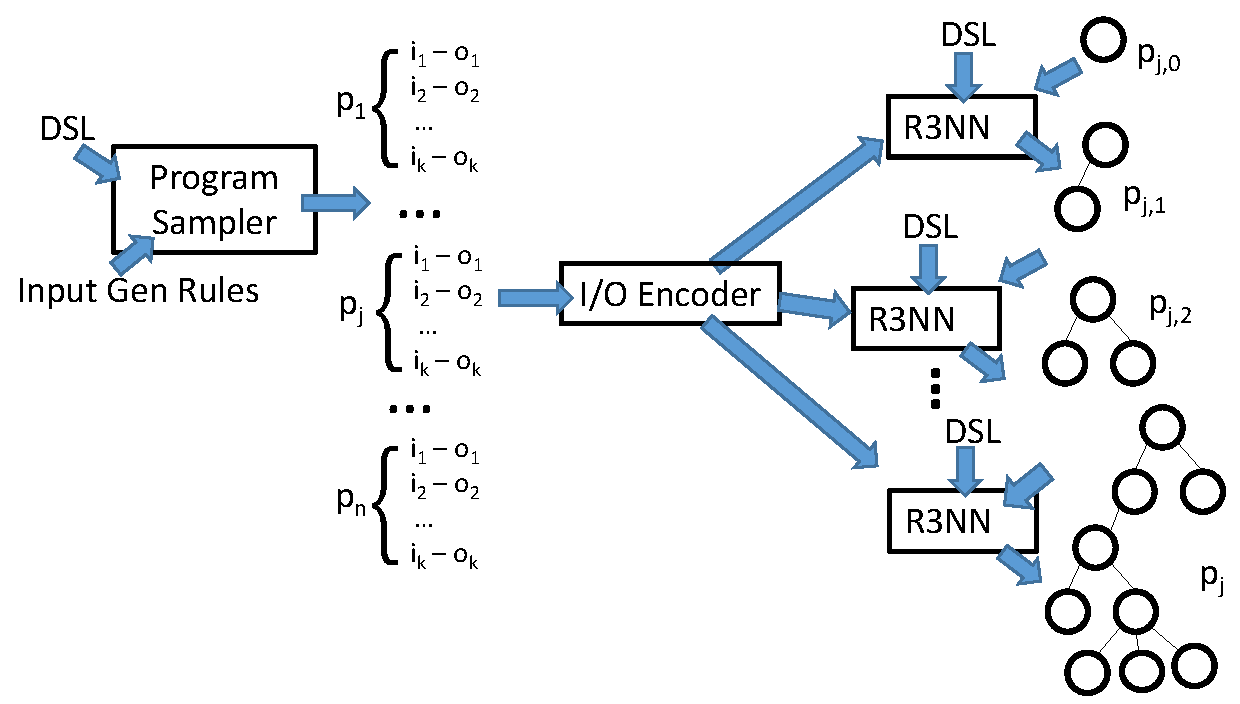
\includegraphics[scale=0.3]{figures/nsps_training.pdf}
        \end{minipage}
        &
        \begin{minipage}{0.5\linewidth}
            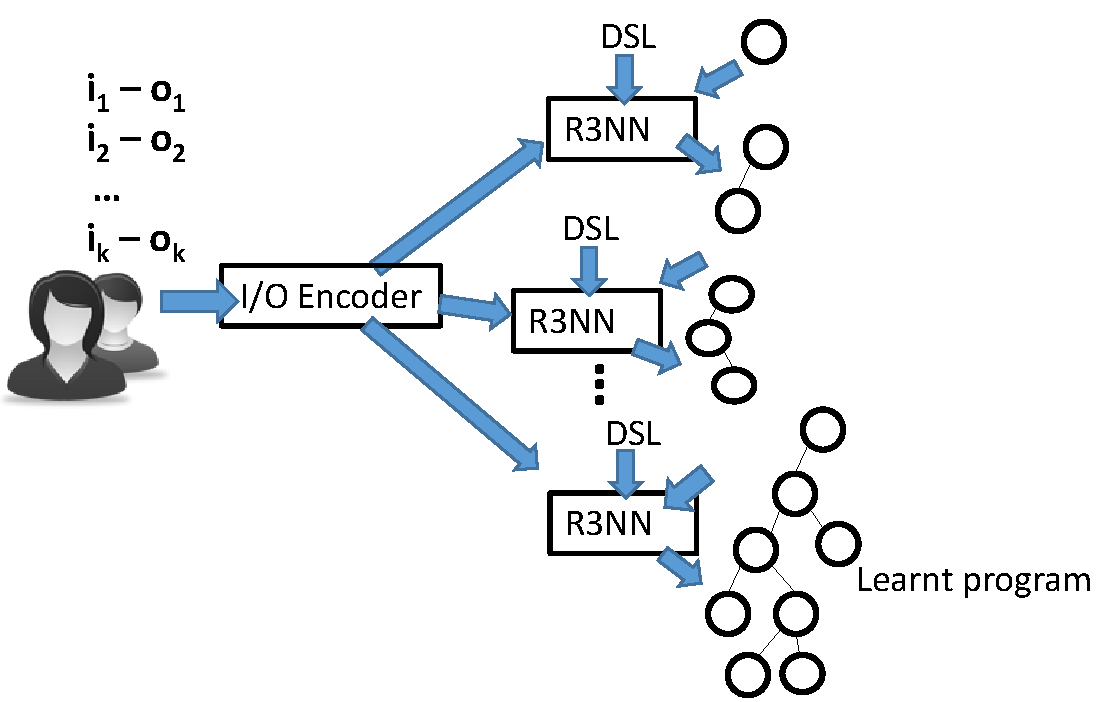
\includegraphics[scale=0.3]{figures/nsps_test.pdf}
        \end{minipage}
        \\
        (a) Training Phase & (b) Test Phase
    \end{tabular}
    \caption{overview of the Neuro-Symbolic Program Synthesis model~\citep{nsps}}
    \label{nsps}
\end{figure*}

\citet{nsps} try out different example encoders,
each embedding into a continuous space a \emph{one-hot} representation of the input or output strings of their domain.
starting out with a simple LSTM baseline,
% but progressing through various versions of a \emph{cross-correlation encoder},
then introducing different variants based on the \emph{cross-correlation}~\citep{bracewell1986fourier} between inputs and outputs.
% sliding the output and input feature blocks over one another to calculate their \emph{cross-correlation}~\citep{bracewell1986fourier},
% then aggregating these by sum or concatenation,
% % using LSTMs instead of dot products then summing,
% then using two more involved approaches using LSTMs.

The baseline sample encoder processes input/output strings of example pairs
using two separate deep bidirectional LSTM networks.
For each pair, it then concatenates the topmost hidden representation
at every time step to produce a $4HT$-dimensional feature vector per I/O pair,
where $T$ is the maximum string length for any input or output string,
and $H$ is the topmost LSTM hidden dimension.
It then concatenates the encoding vectors across all I/O pairs
to get a vector representation of the entire I/O set.~\citep{nsps}

% Of these, they found their aggregation by concatenation to only perform on par with their LSTM baseline (both 88\% accuracy on their test dataset) while the sum aggregation performed more poorly (65\%),
% whereas their further additions only made for minor improvements on this (91\% each).
% They additionally empirically test out different times at which to incorporate the input-output conditioning,
% and found pre-conditioning (adding them before the recursive pass) to work best.

\begin{figure*}[h]
    \begin{tabular}{cc}
        \begin{minipage}{0.45\linewidth}
            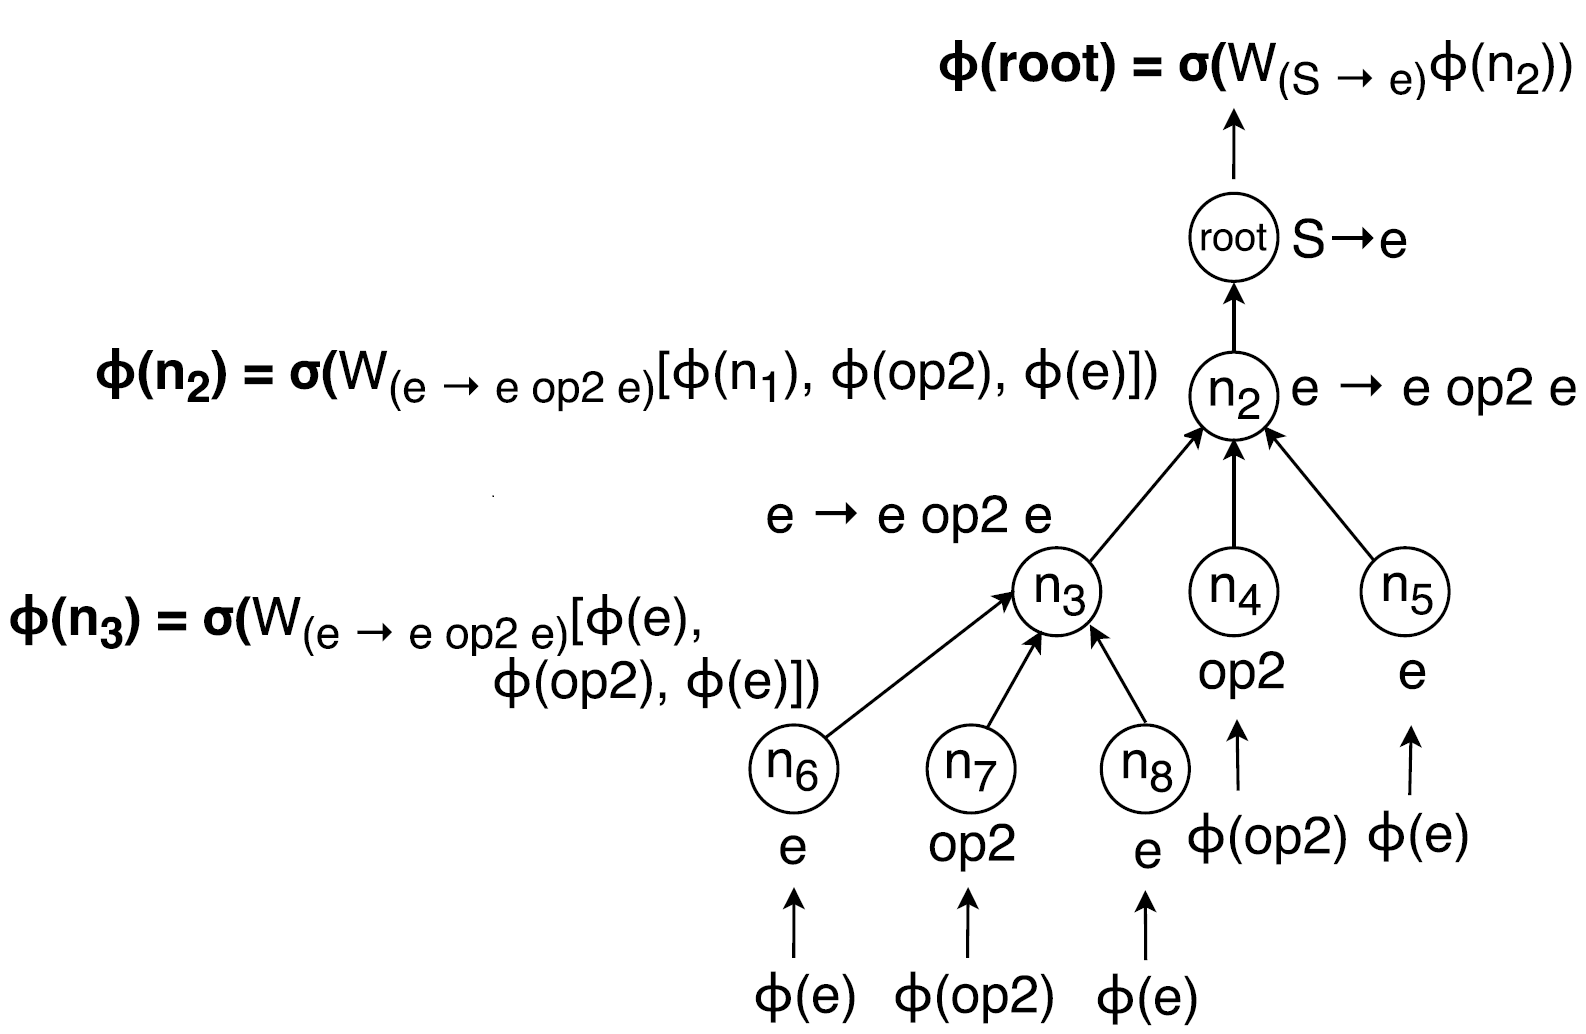
\includegraphics[scale=0.16]{figures/tree2.png}
        \end{minipage}
        &
        \begin{minipage}{0.55\linewidth}
            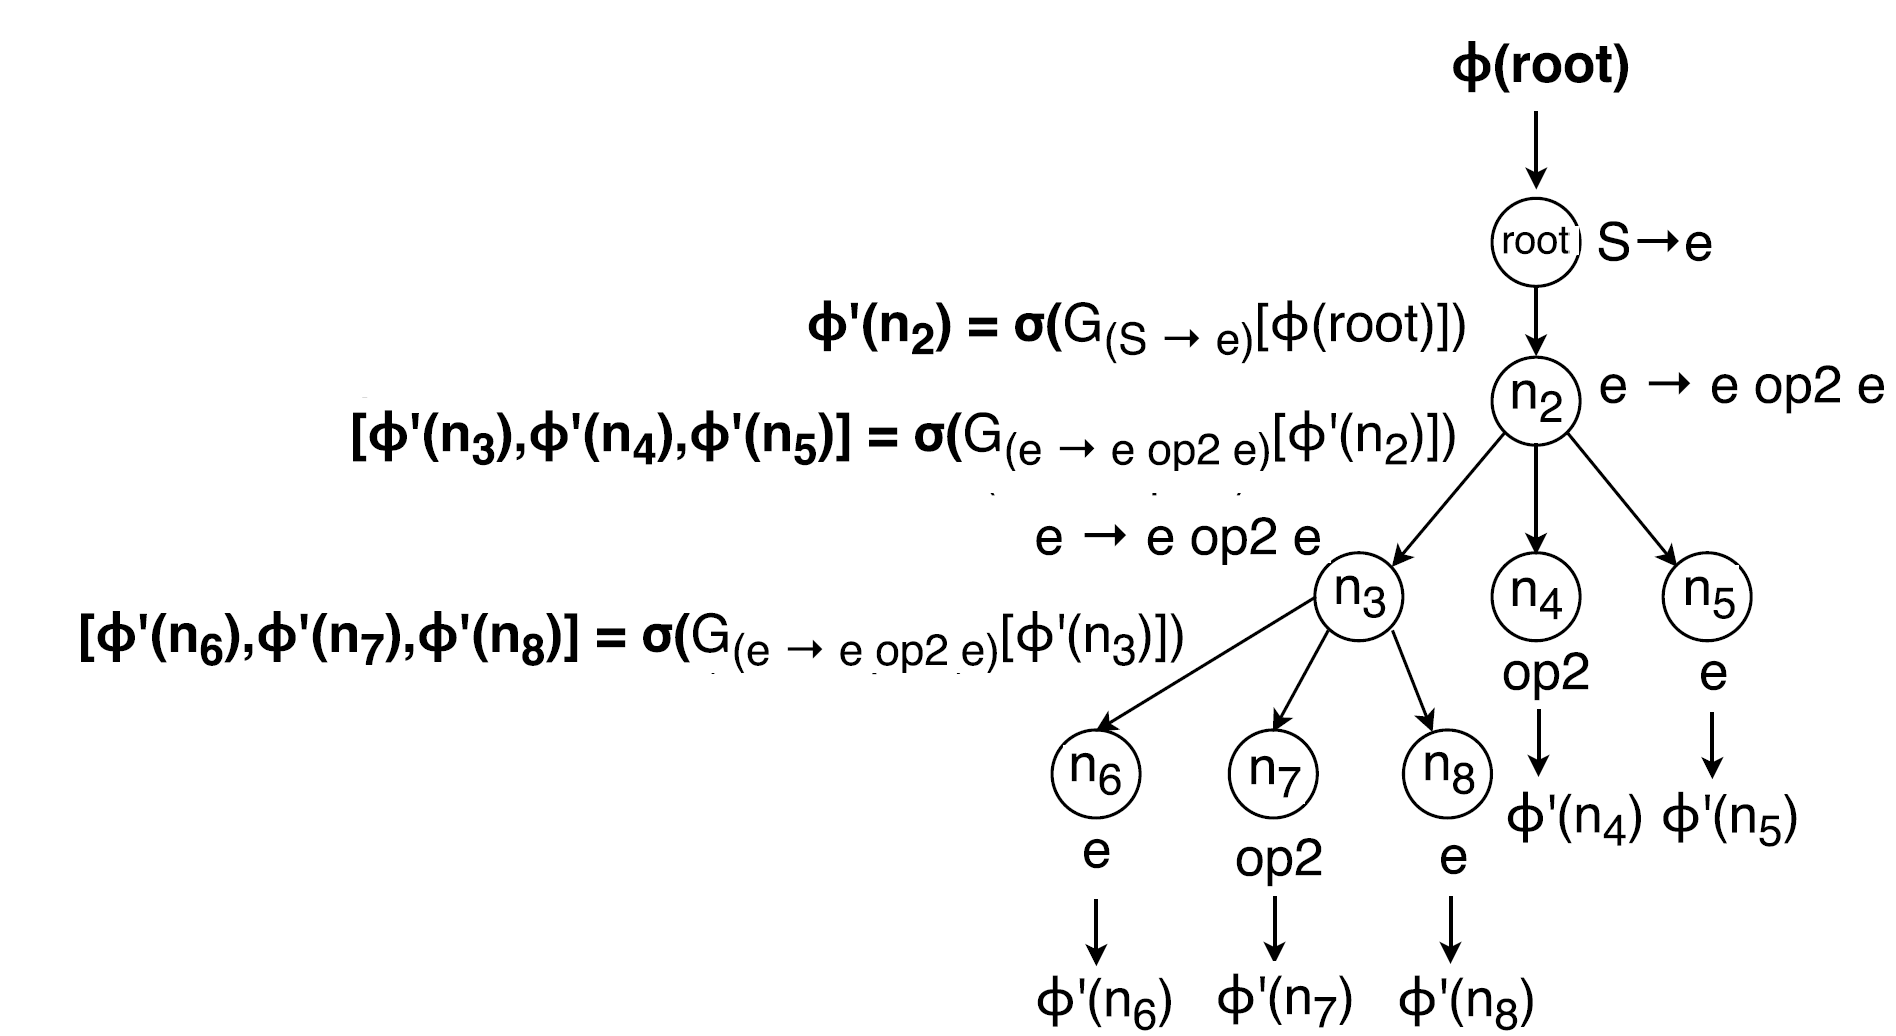
\includegraphics[scale=0.16]{figures/tree3.png}
        \end{minipage}
        \\
        (a) Recursive pass & (b) Reverse-Recursive pass
    \end{tabular}
    \caption{(a) The initial recursive pass of the R3NN. (b) The reverse-recursive pass of the R3NN where the input is the output of the previous recursive pass.}
    \label{r3nn}
\end{figure*}

The workings of the R3NN are illustrated in Figure \ref{r3nn}.
The R3NN utilizes two parallel sets of neural networks,
both consisting of one neural net per grammar production rule $r \in R$,
one set for each of its two passes through an AST: $f_r$ and $g_r$,
in the diagram denoted by $W(r)$ and $G(r)$, respectively,
with $r$ calculated as production rule $R(n)$ of non-leaf node $n$.
These neural networks use only a single layer with hyperbolic tangent activation function (denoted by $\sigma$).

In addition to these, the R3NN has a representation $\phi(s) \in \mathbb{R}^M$ for every symbol $s \in S$,
and a representation $\omega(r) \in \mathbb{R}^M$ for every production rule $r \in R$.

The R3NN first makes a \emph{recursive pass} from the embeddings $\phi(l)$ of leaves $l \in L$ of the program tree through neural networks $f_r$ at each branch,
mapping from $Q \cdot M$ to $M$ dimensions,
i.e. from concatenated right-hand side (RHS) vectors to a left-hand side (LHS) vector,
all the way to the root node of the partial program,
making for an embedding $\phi(root)$ of the full program so far.

$Q$ here represents the number of child nodes of the branch in question
(as dictated by the grammar expansion rule it represents),
while $M$ indicates the number of features used per AST node.
At any leaf $l \in L$, $r$ is determined by its symbol $s \in S$
representing an operator in the DSL, calculated by $S(l)$.

It then performs a \emph{reverse recursive pass} from this root embedding $\phi(root)$,
now passing back to the leaves through $g_r$,
one of a second set of neural networks,
mapping back from $M$ to $Q \cdot M$ dimensions,
i.e. from a LHS vector back to concatenated RHS vectors $\phi'(c)$ for any node $c$,
which now have their individual embeddings instilled with structural information about the entire program and how they fit into this larger structure.

In the event a node $c$ constitutes a non-leaf node $n$,
this process is then repeated, until reaching leaf embeddings $\phi'(l)$.
Such leaf embeddings $\phi'(l)$ are now different for leaf nodes sharing the same symbol,
while before these two passes their original embeddings $\phi(l)$ would have been identical.

\citet{nsps} define an \emph{expansion} $e \in E$ as a combination of a hole (non-terminal leaf node) $e.l$ and a grammar production rule $e.r$, together making up for a way we can expand our PPT.
Expansion scores of an expansion $e$ they define as $z_e = \phi'(e.l) \cdot \omega(e.r)$.

These scores are then normalized to probabilities using a \emph{softmax} operation.
They find processing leaf embeddings $\phi'(l)$ by a bidirectional LSTM before the score calculation helped as well.

To condition R3NN expansion probabilities on the input-output examples specifying desired program behavior in PBE,
\citet{nsps} test different places in the R3NN to add these,
but settle on concatenating them to the node features $\phi$ before the recursive pass.

For the training phase they use the simple setup of supervising by the \emph{task function},
i.e. the function we aim to synthesize,
while for the test phase they sample 100 programs from their trained model.
They consider the synthesized program to have passed if any of these demonstrate the correct behavior on input/output.

% misc

Some critiques of this model have included it being harder to \emph{batch} (i.e. enable parallel execution) over multiple task functions for larger programs due to its tree-based architectures,
as well as its pooling at the I/O encoding level being harder to reconcile with \emph{attention} than models using \emph{late pooling}.~\citep{devlin2017robustfill}

For our purposes, by merit of the untyped Microsoft Excel \emph{FlashFill}~\citep{prose} domain this model was tested on,
it also shares a weakness with other neural synthesis models:
as neural synthesis models have usually been applied to untyped domains,
they have not been augmented to use information on types,
while existing type-theoretic synthesis approaches have shown this info to be highly valuable.

\paragraph{Neural-guided search} \label{sec:ngs}

\emph{Neural-guided search} is an another approach to \emph{hybrid} neural synthesis,
like \citet{nsps}'s \emph{neuro-symbolic program synthesis} model combining symbolic and statistical synthesis methods.~\citep{nps}
It employs neural components to indicate search order within traditional search methods
such as enumerative search (possibly pruned using deduction),
'sort-and-add' enumeration or sketch filling.~\citep{deepcoder}

\citet{kalyan2018neural} built on this to extend the guidance to each search step,
integrating \emph{deductive} search (e.g. a SAT/SMT solver, extensions
like \emph{conflict-driven} learning~\citep{feng2018program}),
a \emph{statistical model} judging generalization,
and a heuristic search controller deciding which of the model's suggested branches
to explore (branch-and-bound~\citep{kalyan2018neural}, beam search%
~\citep{polosukhin2018neural}, $A^{*}$~\citep{lee2018accelerating}).
The statistical model mentioned here is where other
neural synthesis methods would fit into this approach.
Another important decision here is when to \emph{prune} branches,
although near the leaves this check may be slower
than to just explore any that remain.~\citep{polozov}

\citet{feng2018program} expanded on neural-guided deductive techniques
like SMT solvers by \emph{conflict-driven} learning,
ensuring that if e.g. a \emph{map} operation would yield an
output list length not corresponding to the desired length,
other operations suffering from the same issue such as
\emph{reverse} and \emph{sort} would be automatically ruled out as well.

\citet{zhang2018leveraging} focus on incorporating deduced constraints
into the statistical model, to allow taking this info into account
in the decision of which branches to focus on.
Another similar effort has been that of \citet{odena2020learning},
which adds additional features describing properties of a function.
Types however have so far been missing here.

Compared to other neural methods, neural-guided search seems
more of a complementary than a competing effort.
The engineering involved to conciliate the benefits of
different approaches here may be quite involved, and as such
are likely less common in research papers comparing neural components,
but their benefits in production systems seem clear.

\section{Background} % \label{sec:background}

In order to test our hypotheses,
we would like to still quickly explain two additional topics before moving on two our own methodology:
\emph{lambda calculus}, which forms the basis for a simple DSL,
as well as \emph{static typing},
which is the topic of our investigation within neural program synthesis.

\subsection{Lambda calculus} \label{sec:lambdacalc}

Whereas modern programming languages might have a broad plethora of grammatical constructs available,
for the purpose of our proof-of-concept we will opt to hide much of this.

Types are most powerful in a setting where the underlying DSL is loosely-constrained,
that is, permits arbitrary type-safe combinations of subexpressions,
such that checks be deferred from the grammar to the type level.
In other words, to keep things simple,
our DSL should ideally support such a notion of an expression,
but preferably as little else as possible.

This brings us to the \emph{lambda calculus}~\citep{lambdacalculus},
the simplest~\citep{selinger2008lecture}
\emph{Turing-complete}~\citep{turing1936computable} grammar
in terms of number of grammar expansion rules.
The lambda calculus requires only three grammatical categories:
variables, function definition, and function application.

% One simple example showcasing all three of these is (($\lambda$x.x) z).

% Working from the inner expression ($\lambda$x.x),
% we have a function definition that given a parameter that we will name $x$, will return the value $x$.
% Our outer expression (($\lambda$x.x) z), then,
% invokes a function \emph{application} on this function,
% using as its sole argument the variable $z$.
% $z$ will then be bound to the value of the parameter $x$.
% To reflect this, we may rewrite the function body $x$ by substituting parameter $x$ with $z$.
% Our full expression has at this point been simplified to just $z$,
% yielding our final result.%
% % ~\footnote{
% %     Simplifying by function application this way is also known in the lambda calculus as $\beta$-\emph{reduction},
% %     corresponding to \emph{local reducibility} in \emph{natural deduction}~\citep{gentzen1935untersuchungen}.
% % }

% Understanding the basics,
% it would be illuminating to go over a slightly more involved example (($\lambda$x.$\lambda$y.$\lambda$z. + x y) 1 2),
% including a binary arithmetic addition operator $+$ taken two arguments of a numeric type,
% two actual numeral literals we will use as arguments,
% and three nested functions with respective parameters $x$, $y$, and $z$.%
% ~\footnote{
%     It may initially seem surprising that this grammar only directly describes \emph{unary} function application.
%     However, if one recalls the \emph{currying} aspect of the lambda calculus,
%     this should not come as a surprise: after all,
%     applying multiple parameters to a function in one go
%     is equivalent to applying them one by one.
% }

% As before, our main expression is a function application containing two parameters, $1$ and $2$,
% which we will apply left-to-right.
% Applying our first argument, substituting our parameter $x$ with $1$,
% we obtain (($\lambda$y.$\lambda$z. + 1 y) 2).
% Applying our second argument, substituting $y$ with $2$,
% we then get ($\lambda$z. + 1 2).
% No longer having any symbolic variables in our inner function application now,
% we can now simplify it, leaving us with ($\lambda$z. 3),
% i.e. a unary function ignoring its sole parameter value to return $3$.

% What this example demonstrates is the concept of \emph{currying}~\citep{currying},
% that is, the ability to separately apply function arguments without our function necessarily being applied \emph{fully}.%
% % ~\footnote{
% %     This is in contrast to functions in e.g. traditional programming languages such as \emph{C},
% %     where a function with two parameters could only be \emph{fully applied},
% %     that is, applied with both of its parameters at once.
% %     And in fact, currying requires a language to support functions as \emph{first-class citizens},
% %     i.e. allowing to use functions as function arguments or return values.
% % }
% As such, a \emph{curried} version of a function is not unlike its original form,
% yet allowing arguments to the function to be applied to it one at a time.
% The way this works is that, when an argument is applied to a curried form of a function taking two parameters,
% the result is a function that still takes one parameter, before yielding the actual result of the original function.
% This is particularly useful to \emph{compose} existing functionality,
% and this idea of functions operating on other functions is also called a \emph{combinator}.

With this lambda calculus, we now have a solid basis for a simple expressive grammar that allows us to defer most checks from the grammar to the type level.%
~\footnote{
    As an interesting coincidence,
    using this as the basis of our synthesis target language means
    we will use an implementation of \citet{lambdacalculus}'s lambda calculus
    to address \citet{church1957applications}'s problem of synthesizing programs.
}

\subsection{Complementing synthesis grammars with \emph{static typing}} \label{sec:statictyping}

Of our goals of expressiveness versus a limited search space,
\emph{types} would seem able to help us primarily in limiting our search space:
we would like them to prune out any parts of the search space that are not sensible,
i.e. would not pass a type-check.

As we have laid out above,
types are nearly a \emph{free lunch} when it comes to restricting the synthesis search space,
as per our hypothesis \#1
% \ref{hyp:types}
thereby improving synthesis performance.
% While static typing would therefore facilitate automation of programming,
% % static typing, as one step toward formal verification,
% this symbiosis works two ways:
% by encouraging the use of statically typed languages,
% type-driven synthesis
% brings the additional advantage of helping reduce the
% risk of potentially costly software failures.%
% ~\citep{miller2018smart,leveson2001systemic}

% \subsubsection{Types versus grammar: generics} \label{sec:generics}

However, one might note here that traditionally,
search spaces in program synthesis have been restricted not using types,
but using \emph{context-free grammars},
% an approach that is the subject of the
as in the
\emph{Syntax-Guided Synthesis competition} (SyGuS-Comp)~\citep{sygus}.
One might wonder: how then would restrictions based on
types compare to restrictions imposed by a grammar?

In a \emph{monomorphic} type system,
containing only simple (unparametrized) types such as \emph{boolean} or \emph{integer},
restraining a search using types is in fact \emph{equivalent}
to a grammar where types are used as symbols in the grammar.%
% ~\footnote{
%     One might note that this equivalence does not imply
%     that neither of these approaches is preferable:
%     it in fact means that a simpler and more generic grammar
%     may achieve the same thing without losing expressivity,
%     allowing better reuse of logic.
% }

However,
% although static typing has been around since the days of \emph{Fortran},
what makes the use of types different from,
and more powerful than grammars in restricting the search space,
is the use of \emph{parametric polymorphism}, i.e. availability of \emph{type variables}:
a function \emph{append} may work using either lists of numbers or lists of strings.%
% ~\footnote{
%     Left out of scope here are \emph{refinement types},
%     which further aid synthesis based on conditions to express e.g. `natural numbers greater than $5$'.
% }
As such, its type signature may be made \emph{generic} such as to have its return type reflect the types of the parameters used.
% Similarly, an \emph{identity} function could work on any type, simply returning its input values.

Having such information available at the type level may add additional information over what is used in the simpler case above.
For example, a function to look up elements in a list based on their respective locations might take as its inputs one list containing any type of element, along with a second list of integers containing the indices.

Now, in a \emph{context-free} grammar,
such distinctions could not be expressed in a meaningful way:
% while one might initially attempt to patch this by enumerating the different options for any parametric types upgraded to left-hand symbols in the grammar,
% with the addition of new operations, types, parametric types, and higher-order parametric types,
such a grammar would quickly explode to the point of no longer remaining a reasonable abstraction to a human observer.
% suddenly a hypothetical \emph{identity function} in the grammar, for one,
% would need to be duplicated at the left-hand-side (LHS) level of the grammar for every known type in the grammar,
% including for potential parametric types (list of booleans, list of integers, list of lists of booleans, \dots).

As such, one may regard the reliance of types over a grammar for the purpose of restricting the search space as a generalization of solely relying on a grammar for the purpose of restricting the search space.%
~\footnote{
    Nevertheless, it should be noted here that not all programs benefit from this,
    but only those for which potential building blocks (or \emph{operators}) do in fact include statically typed functions making use of either parametric return types, that is to say, return types containing type variables.

    As a result, this restriction limits our method from adding value in direct synthesis of programming languages that are \emph{dynamically typed},
    e.g. the language Ruby, as well as those lacking \emph{parametric polymorphism}, e.g. the language Go.

    However, this only partly hinders those wishing to synthesize programs in such languages:
    rather than synthesizing in such languages directly, we would suggest synthesizing from the language that \emph{best constrains} the search space,
    then using source-to-source translation methods as discussed in Section
    % \ref{sec:source2source}
    \ref{sec:synthtypes}
    (e.g. neural machine translation~\citep{kalchbrenner2013recurrent}),
    using the synthesized program as input to obtain a program translated into the target language.
}

% \subsubsection{Types versus expressiveness}

% However, in order to nevertheless achieve a high degree of expressiveness,
% we simultaneously require a type system powerful enough to model any logic we might wish to utilize.

% Now, in order to further constrain our search space as much as possible,
% we would generally prefer to have our functions be as generally applicable as possible.

% So far the best attempts at generalizing functionality in programming languages has taken after the abstractions discovered in \emph{category theory}~\citep{eilenberg1945general,awodey2010category},
% a branch of mathematics 
% % priding itself in generality to the point where it has earned the moniker \emph{abstract nonsense},
% formalizing mathematical structure,
% which defines abstract categories based on their defining properties.

% The implication of this is that functions often used on a list structure,
% such as \emph{map} or \emph{traverse},
% would no longer be defined to take \emph{list}s,
% but to instead operate on the more abstract categories of \emph{functor} and \emph{traversable},
% both of which would the \emph{list} data structure would be a \emph{member} of,
% generalizing their area of applicability to extend to other data structures as well.

% Such abstractions will require a type system supporting constructs such as \emph{type classes}~\citep{blott1991type}.
% This requirement narrows down our potential choice for a synthesis language to a select number of languages,
% including Haskell, Clean, Rust, Mercury, Scala, Coq, Agda, and Idris.

% \paragraph{Typed holes} \label{sec:holes}

% In the context of program \emph{sketches} and \emph{partial programs} we had previously discussed the concept of \emph{holes},
% i.e. the missing parts of a program that a synthesizer would still need to fill out.
% in Section \ref{sec:challengesnps} we had also mentioned the challenge of how traditionally we were only able to evaluate the quality of \emph{complete} programs.
% Now, as a compromise in lieu of such a proper behavioral evaluation of a complete program,
% we would like to be able to perform a \emph{type check} by means of a rudimentary provisional sanity check%
% % ~\footnote{
% %     While we are using our simple training setup using \emph{strong supervision},
% %     we cannot technically \emph{train} on \emph{compile checks} as a feedback signal yet,
% %     but at the very least we can already \emph{filter} on such compile checks during \emph{evaluation}.
% % }
% to filter on during evaluation.

% Now, using most statically typed languages,
% for the purpose of such a type-check we could simulate such holes by means of a \emph{dummy value}.
% Many programming languages offer e.g. \emph{undefined} or \emph{null} values for this purpose,
% and these will allow us to write an incomplete functional program template,
% yet at the same time pretend our partial program is in fact \emph{complete}.

% A more elegant solution for our purposes here is proper language support for such \emph{typed holes}~\citep{hashimoto1997typed},
% as available in Agda~\citep{holesagda},
% Idris~\citep{holesidris},
% and Haskell~\citep{holeshaskell}.%
% ~\footnote{As we will explain later, each of these languages are implementations of the \emph{lambda calculus}.}
% Typed holes enable type inference for any such holes,
% in turn enabling suggested completions to the user.
% Such interactive program synthesis has been labeled as the solver-aided
% programming method \emph{sketching}~\citep{gulwani2017program} or
% \emph{type-driven development}~\citep{typedrivendev}.

% As such, one of our goals is to improve suggested hole completions in such languages to facilitate this interactive programming style.
% On the other hand, we may also hook into such existing completion logic to inform our synthesizer.

% \pagebreak

\section{Methodology} % \label{sec:methodology}

In this section we will discuss our program synthesis model,
which applies type information to improve synthesis quality in programming by example.

We further explain how this synthesizer builds upon the work of \citet{nsps},
the functional programming synthesis DSL we use with this to exploit its features,
as well as how we generate datasets in order to obtain training and test sets in our DSL.

To explain the design decisions we made,
we will go by the synthesizer taxonomy of \citet{gulwani2017program} introduced in Section \ref{sec:litreview}.
The first two points criteria, i.e. constraints on expressions of user intent and search space,
together give the background needed to understand both our dataset generation method as well as the synthesizer itself.

We will therefore first explain our design decisions with regard to these,
then continue to lay out the design of our dataset generation method and synthesizer.

One should bear in mind that our goal here is not to create the perfect production-ready synthesizer;
instead we will aim to answer each of these categories with the question:
what is the simplest way in which we might effectively test our hypotheses?

\subsection{User intent}

User intent in program synthesis can be expressed in various forms, including logical specification~\citep{temporalstreamlogic} (among which \emph{types}~\citep{synquid}),
input-output examples, traces, natural language~\citep{abstractsyntaxnetworks},
partial programs, or even related programs.~\citep{gulwani2017program}

For our expression of user intent, we would like to use input-output examples,
which may be considered a compromise between what is easier for the end-user,
who may ideally prefer natural-language descriptions of program behavior,
versus what is easier for the synthesizer,
which may ideally prefer a complete formal specification of program behavior.

This puts us in the field of programming by example (PBE),
which has a broad area of application despite being conceptually simple%
% ~\footnote{
%     Although arguably the potential applications of synthesis from natural-language descriptions are even broader,
%     % in terms of computational requirements and dataset generation it is a much harder problem.
%     one more challenging aspect about it is that we do not generally have an automated way of evaluating if a given program satisfies the natural-language description,
%     essentially limiting training to using strong supervision.
% }.
.

To (1) reduce ambiguity, (2) increase result quality, and (3) speed up synthesis, a synthesizer may be passed more information in various ways:
\begin{itemize}
    \item additional data within the same mode of user intent, e.g. further input-output examples;
    \item an additional expression of user intent of a different type, e.g. a natural language description~\citep{polosukhin2018neural} or type signature of the desired function~\citep{myth};
    \item more descriptive types~\citep{synquid};
    \item additional features describing properties of the function~\citep{odena2020learning}.
\end{itemize}

Of interest here is the realization that, in modern programming languages, types may be \emph{inferred} even without explicit type annotations.
% implication: language preferably should have type inference
This is then a hidden benefit of synthesis from input-output examples:
if the types of input-output example pairs may be \emph{inferred},
then we may regard this as free additional information we can incorporate in our synthesis process.%
~\footnote{
    Optionally, it may be of interest to allow users to,
    in addition to the function types implied in their input-output examples,
    still let them explicitly clarify their desired function type manually as well.

    While on first glance this may seem potentially redundant with input-output pairs,
    it may actually help to constrain the potential function space to a sufficiently general form,
    benefiting both the user,
    by yielding a mode widely-applicable function,
    while also benefiting the synthesizer,
    by helping to constrain the search space.
}

\subsection{Program search space}

The program search space consists of the synthesis language (defined by a \emph{context-free grammar}),
either general-purpose or a \emph{domain-specific language} (DSL),
potentially further restricted to a subset of its original operators,
such as by providing a whitelist of \emph{operators}.

The trade-off here is one of expressiveness (can we write a satisfactory program, ideally using not too much code?) versus limiting our search space (ensure we can find a solution within too long).

So, how does this fit into our question on reaching a configuration that could best demonstrate the use of types?
Now, providing empirical evidence on how every design choice impacts the usefulness of type information is not in scope for this thesis.
Instead, we will make informed guesses
% for some of the decisions involved here (language, grammar subset) to provide us with some level of flexibility,
% then use that flexibility at the operator level and generate different datasets from these, to nevertheless provide empirical evidence on the effect of some other decisions here (how do various properties of type signatures affect the usefulness of type information?).
to pick our language, grammar subset and operator set.

Not having empirical evidence to guide our design decisions upfront, however,
we appear free to take some guidance from program search space considerations to generally improve synthesis efficiency:
how might we achieve the highest amount of expressiveness within a limited search space?
The answers we have found to this question, we argue,
is intuitively in line with a program search space designed to demonstrate the utility in synthesis of type information.

Under this goal, it would seem preferable to pick a limited grammar in the functional programming paradigm using static typing.
In the following sections we will lay out how we have reached this conclusion.

\subsubsection{The functional programming context}

% \begin{figure*}[h]
%     \begin{tabular}{c|c}
%         \begin{minipage}{0.5\linewidth}
%             \begin{center}
%                 \huge{$\lambda x . x$}
%             \end{center}
%         \end{minipage}
%         &
%         \begin{minipage}{0.5\linewidth}
%             \begin{center}
%                 \huge{$f \circ g$}
%             \end{center}
%         \end{minipage}
%         \\
%         (a) lambda function representing the identity function & (b) function composition
%     \end{tabular}
%     \caption{function definition and composition, two of the central concepts in functional programming}
%     \label{fp}
% \end{figure*}

The \emph{functional} paradigm,
named after the \emph{pure} functions of \emph{mathematics},
has been characterized by its composability or \emph{modularity}~\citep{hughes1989functional},
which is key in the creation of synthesizers that generalize well,
as it encourages \emph{reusing} existing abstractions to allow for a large expressivity using only a small vocabulary,
matching our synthesizer search space requirement of maintaining \emph{expressiveness} while limiting our \emph{search space}.

In addition, functional programming offers various general-purpose programming languages,
which helps potentially make our synthesizer potentially applicable to a wide variety of domains.
It is also well amenable to programming \emph{types},
% allowing advanced constructs such as
% algebraic datatypes (ADTs)~\citep{burstall1977design},
% generalized algebraic datatypes (GADTs)~\citep{dybjer1991logical},
% and, more importantly for our purposes, type classes~\citep{blott1991type}.
% While \citet{haskellhistory} provides an overview of these,
% the point for our purpose is that these features contribute to expressiveness,
% and simultaneously,
which help reduce the search space in program synthesis.

The basic abstraction in functional programming is the \emph{function}.
This means we would view our synthesized programs as being and consisting of \emph{pure functions}~\citep{fortran95},
i.e. returning a deterministic output for any given inputs,
without performing any additional side effects.%
~\footnote{
    These properties of determinism and lack of side effects are generally taken as prerequisites in \emph{programming by example},
    as we will verify program behavior by comparing the output of our synthesized output to that of our original task function.

    If \emph{non-determinism} came into play,
    forcing us to test samples of our stochastic function output,
    we would need to extend our synthesis domain to something that could well be called \emph{synthesis by property} instead.

    Synthesizing functions with \emph{side effects} instead appears closer to the domain of synthesis from \emph{traces},
    where the synthesis specification instead consists of a description of such triggered side effects as a function of various user inputs.
}

% The concept of \emph{purity} comes directly from that of the \emph{mathematical function} that this paradigm is named after.
% The nice thing about such a pure function is that it satisfies some properties that make it easier to reason about like \emph{referential transparency},
% which means we may substitute any pure expression with its calculated result,
% % as we will see in Section \ref{sec:lambdacalc}.
% as demonstrated during lambda calculus evaluations.

One may well regard programs in this paradigm as constructed of a (nested) tree of function applications.
One reason we would like to consider such programs of a tree-based form,
rather than as a list of imperative statements such as variable definitions or mutations,
is that the view of programs as function compositions guarantees us that any complete type-checking program from the root,
filtered to the right output type,
will yield us output of the desired type,%
% ~\footnote{
%     Technically this holds for in as far as we our functions are \emph{fully} or \emph{partially} applied to the extent they will give us the desired result,
%     something we will keep in mind when choosing our program \emph{expansion rules} later on.
% }
helping us reduce our synthesis search space to a sensible subset,
devoid of e.g. programs containing variable definitions that end up never being used.

This guarantees that, rather than just branching out,
our search will focus on finding acceptable solutions.
This is to be contrasted with \emph{imperative} programs,
a coding style characterized by variable mutation.
% historically popularized for the purpose of performance optimization from the earlier languages such as \emph{assembly}.
Synthesis for such languages exists as well~\citep{shi2019frangel},
but does not support the use of e.g. type-theoretic approaches,
limiting the synthesis methods we might use here
while giving us less means to constrain our search space.

The functional programming paradigm started with \emph{Lisp},
an implementation of \emph{lambda calculus},
as introduced in Section \ref{sec:lambdacalc},
which has essentially formed the basis for functional programming languages ever since.

We will next discuss 
% how this fits into the language features we are looking for in a synthesis language,
% to then finally use this knowledge to inform
our decision on an actual synthesis language,
followed by a further explanation on how we adapt lambda calculus for our own synthesis grammar.

\subsubsection{Synthesis language}

Our \emph{synthesis} language, or \emph{target} language,
is the language we would like for our synthesizer to generate.
This is as opposed to the \emph{host} language,
i.e. the language that our synthesizer is implemented \emph{in}.
% While these are separate design decisions,
% they are regarded as separate more so in some
% branches of program synthesis than in others.

Neural synthesis methods have often tended to implement custom DSLs as the target language,
while for the host language typically using \emph{PyTorch}~\citep{pytorch}.
% \emph{Python}~\citep{rossum1995python},
% a dynamically typed language that has become popular in the
% data science and machine learning domains as it offered
% easy integration with existing scientific computing codebases
% written in \emph{Fortran}, \emph{C}, and \emph{C++}~\citep{mckinney2012python},
% particularly the \emph{basic linear algebra subprograms} (BLAS)~\citep{lawson1979basic},
% which have formed the basis of the \emph{Numpy}~\citep{oliphant2006guide} tensor library.
% More important for the Python ecosystem in recent years has
% been the introduction of \emph{deep learning frameworks}%
% ~\citep{pytorch,abadi2016tensorflow,jax2018github},
% which built on top of the ideas of Numpy
% to add acceleration using devices able to run computations in parallel,
% including \emph{graphics processing units} (GPUs),
% \emph{application-specific integrated circuits} (ASICs) such as Google's \emph{tensor processing units} (TPUs),
% and \emph{field-programmable gate arrays} (FPGAs)
% including Microsoft's \emph{neural processing units} (NPUs);
% along with \emph{automatic differentiation}%
% ~\citep{neidinger2010introduction,baydin2017automatic}
% to automate implementation of backward passes of
% \emph{backpropagation}~\citep{backproprnn}
% in machine learning models.
For our purposes working with types however,
it would be nice to be able to defer type logic to an existing language.%
% ~\footnote{
%     Ideally, we would like to do this without having to rely on
%     \emph{foreign function interfaces} (FFIs)
%     to glue languages together,
%     a mechanism to use functionality from a different language.
%     % reasons: https://en.wikipedia.org/wiki/Foreign_function_interface#Operation
% }

This idea though would require our host language
to be able to construct ASTs for, compile,
and interpret our \emph{target} language,
while also requiring the availability of a
deep learning framework for our model implementations.

% While we have so far glossed over the intersection
% between type systems and the lambda calculus,
% the \emph{typed lambda calculus},
% by the Curry-Howard isomorphism~\citep{howard1980formulae} corresponding to
% \emph{natural deduction}~\citep{gentzen1935untersuchungen} in logic,
% actually consists of different variants.%
% ~\footnote{
%     On a sidenote, type-level guarantees on the lambda calculus do technically
%     come at the expense of expressiveness in terms of its
%     Turing-completeness~\citep{draheim2017semantics},
%     although this hasn't really prevented it from being put to practical use.
% }

% \citet{barendregt_1991}'s \emph{lambda cube} offers a
% taxonomy of such type systems for the lambda calculus,
% each corresponding to a different branch of logic.
% It is based on the presence of
% \emph{parametric polymorphism}, i.e. parameterized types,
% \emph{dependent types}~\citep{martin1984intuitionistic},
% i.e. types whose definition depends on a value%
% ~\footnote{
%     This variant is called the $\lambda-\Pi$-\emph{calculus}%
%     ~\citep{pym1991proof,milner1992functions,boudol1998pi},
%     combining the lambda calculus with the $\pi$-\emph{calculus}~\citep{engberg1986calculus}.
% },
% and \emph{type operators},
% i.e. the `function' equivalent using types for values.

% Their taxonomy starts with the 
% \emph{simply-typed lambda calculus}~\citep{church1940formulation},
% offering none of these features,
% and ending with the \emph{calculus of constructions}~\citep{coquand1986calculus},
% offering all three.

% Theorem prover \emph{Coq}~\citep{barras1997coq} implements the
% \emph{calculus of inductive constructions}~\citep{huet1987induction},
% a derivative of the calculus of constructions further adding \emph{inductive types}.
% \emph{System F}~\citep{girard1971extension},
% the combination adding only parametric polymorphism,
% also known as the \emph{polymorphic} or \emph{second-order lambda calculus},
% is implemented in \emph{Haskell}~\citep{jones2003haskell} and in
% \emph{ML} dialects such as \emph{Standard ML}~\citep{harper1986standard},
% \emph{OCaml}~\citep{leroy2014ocaml}, and \emph{F\#}~\citep{syme2005f}.
% \emph{Agda}~\citep{norell2008dependently} and
% \emph{Idris}~\citep{idris} add dependent types on top of these,
% corresponding to \emph{second-order predicate calculus},
% putting them only one step away in the cube from the calculus of constructions.
% Further extensions to the lambda cube taxonomy have been proposed as well.%
% ~\citep{berardi1988towards,roorda2001pure,guallart2015overview}

% Any ML-like calculus with algebraic datatypes can serve as a core language for type-driven synthesis.~\citep{gulwani2017program}
% % we can use types without dependent types or type operators as well.

% In summary, our ideal target language is a lambda calculus
% typed to offer at least polymorphic parametrism (System F),
% further offering type inference, and ideally typeclasses
% and typed holes.
% In our host language, we are looking for a deep learning framework,
% along with the ability to construct ASTs for, compile, and interpret our target language.

% Note that the target and host languages may in fact be the same language,
% and in fact, as our host language tasks closely resembly the
% tasks of a compiler or interpreter of the target language,
% for languages featuring \emph{bootstrapped} compilers,
% i.e. written in their own language,
% such tooling in fact \emph{will} likely be most readily available in the language itself,
% potentially making a compelling case for keeping target and host languages identical.

% Given this list of requirements,
% we are seeing a general conflict of interest between
% our requirements of the host and target languages,
% where our target language wishlist would bias us toward more fully-featured languages,
% whereas particularly the host language requirement of a deep learning
% framework would pull us toward the more-established languages,
% as maintaining such a framework is typically a fairly ambitious endeavour.
% Simultaneously, our source language must have the ability to
% manipulate, compile and interpret ASTs from our target language.

% While these stringent requirements appear to have so far commonly deterred
% researchers from combining type-aided synthesis with neural synthesis methods,
% we have found a way to conciliate these requirements
We conciliate these requirements
by using \emph{Haskell}~\citep{jones2003haskell} as both our host and target language,
which is a statically typed, purely functional programming language based on the lambda calculus and featuring type inference,
% and lazy evaluation,
% which further enables dealing with infinite data structures.
%~\footnote{Source: \url{https://wiki.haskell.org/Lazy_evaluation}}
% This configuration turned out to fill every requirement we had,
% while following the use of this language
and has already been in use in various non-neural synthesis papers%
~\citep{synquid,hornclauses,scythe,gissurarson2018suggesting}.%
% ~\footnote{
%     For future researchers interested in expanding synthesis research toward target languages featuring \emph{dependent types},
%     it may be of interest to look into \emph{Agda},
%     which was implemented in Haskell,
%     so should be viable to manipulate and interpret from Haskell as well.

%     While \emph{Idris} had also started out this way,
%     allowing for a similar setup,
%     its second iteration has bootstrapped its compiler,
%     severing the tie with Haskell.
% }
% Of these, perhaps the least obvious was the presence of a deep learning framework,
% as this required us to use a third-party library.

For a deep learning framework, we had evaluated Haskell ports of
\emph{PyTorch} and \emph{TensorFlow}~\citep{abadi2016tensorflow}.
At the moment of choosing, the Haskell port of PyTorch,
named \emph{HaskTorch}~\citep{hasktorch}%
% ~\footnote{
%     HaskTorch has an API essentially modeled after PyTorch, as it is wrapping the same C++ codebase.
%     It additionally features a second parallel `typed' API however,
%     which offers extra static checks of tensor details such as dimensions.

%     While the original API will limit learning curve for those coming from PyTorch,
%     in implementing our (non-trivial) model we found it quite helpful
%     to make use of the typed API for the extra compiler checks.

%     We did run into some learning curve there as well,
%     such as how to dynamically determine hyperparameters
%     which static tensor typing expects to know at compile-time,
%     e.g. to let users pass these as command-line flags,
%     or to search over these as part of hyperparameter optimization.
%     We aim to further lay these out in a future blog post.
% }%
,
turned out the significantly more active of the two,
and along with its welcoming and helpful community solidified our choice.

\subsubsection{Grammatical subset} \label{sec:grammar}

% Now, while the lambda calculus looks like a promising start,
% how does it relate to the simple DSL we seek to test our hypotheses?
% Surely, a language would traditionally require various grammatical constructs to support e.g.
% literal values, variable definitions, infix operators such as the mathematical addition operator $+$, return statements, conditionals, and more?

% Otherwise, however, we will argue that for our purposes,
% we actually need \emph{less},
% not \emph{more} than,
% what is offered by the lambda calculus for the purpose of our \emph{synthesizer} DSL.%
% ~\footnote{
%     We will however allow expressions including arbitrary grammar constructs in our user-defined \emph{operator definitions} ---
%     while we will infer the \emph{types} of these operator definitions and interpret them to \emph{run} our synthesized programs,
%     our synthesizer itself does not need to concern itself with the internals of these definitions,
%     or generate similar definitions itself.
%     The \emph{synthesizer} DSL only needs to concern itself with the grammatical constructs that our synthesizer will actually be tasked with \emph{producing} itself.
% }

% % infix operators such as the mathematical addition operator $+$

% Viewing traditional operators such as \emph{addition} as (curried) functions for one,
% as we have done in Section \ref{sec:lambdacalc},
% can both simplify the way we view things,
% while also increasing expressiveness.
% And in fact, this is indeed what happens in various functional languages,
% where traditional operators such as \verb|+| are viewed simply as infix operator forms of curried functions.

% In Haskell language, for example, \verb|+| may be used to refer to the addition operator in infix notation,
% whereas \verb|(+)| may be used to refer to its form as a traditional function.
% Other languages such as OCaml, Idris and Agda follow a similar pattern.
% In other words, even if we want our DSL to support e.g. arithmetic operations,
% we may just express these using our existing concept of functions,
% rather than adding such functionality at the grammar level.
% For our purposes, we will therefore use such operators simply as functions,
% rather than using them in infix notation.

% % conditionals

% As such, we might express as curried functions not only basic \emph{mathematical} operators,
% but by wrapping them as library functions,
% also traditional \emph{grammatical} constructs as (functional) \emph{conditionals} and function composition operators.%
% \footnote{
%     Whereas for \emph{legibility} purposes, a programmer may prefer to read code using a grammar rich with \emph{syntactical sugar},
%     for the purpose of program \emph{synthesis},
%     it is preferable to decouple the syntax used for synthesis from that presented to the reader,
%     so as to prevent duplication during synthesis to restrict the search as much as possible.
%     Instead, a synthesized program might then be \emph{converted} so as to use a more legible grammar.
%     For the purpose of this thesis, we will not focus on reader-friendly syntax, however.
% }

% % literal values

% To simplify the problem for the purpose of our experiment,
% we would furthermore disallow the use of arbitrary values such as free-style numbers or strings generated by our synthesizer.
% Instead, in order to keep this tractable we will constrain ourselves to user-supplied constants.
% % A proper solution here may involve e.g. \emph{version space algebras} (VSAs).~\citep{mitchell1982generalization}

% % variable definitions

% Having \emph{variable definitions} would primarily allow us to reduce duplication in our program.
% % or in the event of values derived from calculations that are non-deterministic or have side-effects,
% % reuse such values across our program.
% % Since the \emph{programming by example} context (without further generalization) forces us to stick to \emph{pure} functions however,
% % for our purposes, synthesizer-generated variable definitions might at best help reduce duplication.
% Therefore, within our present scope we may settle for accepting this duplication in favor of further simplicity.

% % function definitions

% As a final simplification, we will also leave out the \emph{function definitions} as provided by the lambda calculus.
% Together with not using synthesizer-defined variables, this helps forego additional complications such as variable name hygiene and (optionally~\footnote{
%     Technically, rather than letting the synthesizer actively generate scoped variable definition lists, we could also just have it generate \emph{unscoped} variables. However, to prevent any optional complexity we will skip out on either of these.
% }) variable scope.
% Instead of using such function definitions,
% we would instead like to stick to the simpler \emph{point-free} style.
% In other words, we would like to leave out redundant \emph{variable names} where possible,
% i.e. to go from ($\lambda$x. + 1 x) to just $(+ 1)$.%
% ~\footnote{
%     In lambda calculus this simplification is titled $\eta$-\emph{reduction},
%     corresponding to \emph{local completeness} in \emph{natural deduction}~\citep{gentzen1935untersuchungen}.
% }
% The utility of this point-free style is further amplified by the presence of \emph{currying},
% which allows us to \emph{partially apply} a function,
% then pass its resulting function in a point-free manner.%
% ~\footnote{Restrictions with regard to parameter order here may be further alleviated using \emph{argument-flipping} combinators.}

% All these restrictions should together leave us with a limited wishlist for our grammar:
% referencing variables from our dataset-defined \emph{operators},
% and applying expressions as arguments to functions.
% Note that either of these two also results in an expression.
% Our synthesizer DSL has therefore ended up with the subset of the
% lambda calculus containing only variables and function application,
% yet not function definition.
% Hopefully, our hypotheses may be tested without this additional complexity.

% \subsubsection{Grammar \emph{unrolling}} \label{sec:unroll}

% We had previously discussed that
Our synthesis DSL
% i.e. the grammar to be actively produced by our synthesizer,
only requires a subset of the functionality in the lambda calculus,
that is, function application and referencing variables,
though without function definition.

% As we discussed in Section \ref{sec:holes},
For the purpose of expressing \emph{partial} programs,
one feature missing in the lambda calculus that we will need to add in our DSL is that of \emph{holes},
ideally \emph{typed} (whether explicitly or implicitly) just as the rest of our programs.

% As a result, our Haskell-based grammar ends up looking as follows:
% \begin{tabular}{ccccc}
%     type & constructor & Type Parameters & example & note \\
%     Exp & App & Exp Exp & exp exp & \\
%     Exp & ExpTypeSig & Exp Type & exp \textbf{::} type & \\
%     Exp & Paren & Exp & \textbf{(}exp\textbf{)} & \\
%     Exp & Var & QName & qname & \\
%     % Type & TyApp & Type Type & Type Type & \\
%     % Type & TyCon & QName & QName & \\
%     % Type & TyFun & Type Type & Type \textbf{->} Type & \\
%     % Type & TyVar & Name & name & \\
%     % QName & UnQual & Name & name & redundant \\
%     % QName & Special & SpecialCon & specialCon & redundant \\
%     % Name & Ident & & ident & \\
%     SpecialCon & ExprHole & & \textbf{\_} & \\
%     % SpecialCon & ListCon & & \textbf{[]} & \\
%     % Exp & Lambda & [Pat] Exp & \textbf{\textbackslash} patt1 patt2 ... \textbf{->} exp & lambdas \\
%     % Pat & PVar & Name & name & lambdas, redundant \\
%     % Exp & Let & Binds Exp & \textbf{let} binds \textbf{in} exp & lambdas typed without ScopedTypeVariables \\
%     % Binds & BDecls & [Decl] & decl1\textbf{;} decl2\textbf{;} ... & lambdas typed without ScopedTypeVariables \\
%     % Decl & PatBind & Pat Rhs (Maybe Binds) & pat \textbf{=} rhs & lambdas typed without ScopedTypeVariables \\
%     % Rhs & UnGuardedRhs & Exp & exp & lambdas typed without ScopedTypeVariables, redundant \\
% \end{tabular}

An attempt to express our DSL
as a \emph{context-free grammar},
taking inspiration from the notation of \emph{extended Backus–Naur form} (EBNF)~\citep{standard1996ebnf},
might look as follows,
where the root node may be either \emph{paren} or \emph{expr}:%
~\footnote{
    One may note that function application here is \emph{unary} in its number of parameters, as it is in Haskell,
    meaning that multiple-parameter functions must be emulated using a chain of such applications.
    \citet{nsps}'s R3NN, however, presumes nodes may in fact have multiple child nodes.

    Using the R3NN on our DSL then means that we must break \citet{nsps}'s original
    assumption that each branch node itself corresponds to one rule expansion,
    as rule expansions may in our case then span multiple AST branch nodes.
    Despite this shift, the theory of R3NN still applies, however.
}

\begin{verbatim}
paren = "(", expr, ")";
expr = paren, " ", paren;
expr = <any variable contained in our whitelisted operators>;
\end{verbatim}

As such, given an operator list consisting of operators \emph{and} and \emph{false},
we would then obtain the following EBNF:

\begin{verbatim}
paren = "(", expr, ")";
expr = paren, " ", paren;
expr = "and" | "false";
\end{verbatim}

Now, in practice, we would like to support using different operator sets
rather than just the one hard-coded for illustrative purposes above,
so it is fortunate we did not need to fix these at the grammar level itself.

However, this simple grammar can unfortunately still generate some bad programs:
\begin{itemize}
    \item programs where the argument of a function is not of the right type.
        This class of mistakes we are no longer able to reliably solve
        at the grammar level due to our polymorphic parametrism.
        Instead, we wish to define this kind of check to the \emph{type} level.
    \item programs where the arity of a given operator is not respected, i.e.
        by invoking more \emph{function applications} than we up-front know are supported.
\end{itemize}

The latter problem we can deal with in either of two ways:
\begin{itemize}
    \item we ignore the problem by deferring it to the type-level,
    providing a solution consistent with how we handle problems of the former type.
    \item we reframe the grammar by statically \emph{unrolling} any provided operators such as to ensure only valid function arities are supported.
\end{itemize}

We consider the second option to be preferable from the synthesizer perspective;
although this would expand the number of production rules in the grammar,
different numbers of function application for a given operator yield different \emph{result types}.
For a type-based synthesizer, distinguishing these makes sense,
as this distinction should facilitate learning.%
~\footnote{
    This view is still up for empirical validation.
    An alternative view may be that a function argument with an unknown type,
    resulting in reduced operator confidence,
    would simply lead a synthesizer to prefer filling a different hole.

    Moreover, the \emph{unrolled} grammar approach implies upfront known arities of functions' argument and return types%
    % ~\footnote{
    %     For in as far as one may speak of arities in a language based on the lambda calculus
    %     using a synthesizer grammar specifically modeled after the lambda calculus.
    % }
    ,
    which is not in fact the case for generic functions like the \emph{identity function},
    which may take and return e.g. numbers but also other functions,
    and more importantly, for functions such as the \emph{argument flipping} combinator
    as well as for the \emph{function composition combinator},
    both of which may operate on functions of any arity.

    This poses a significant limitation for the unrolled approach:
    it essentially means such arity-agnostic combinators are not supported,
    which in the context of functional programming feels like an undesirable limitation.

    While we acknowledge the limitations of this present approach,
    considering the operator set we would like to use in our experiments,
    which we will introduce in Section \ref{sec:task},
    we will consider this as sufficient for the purpose of our present paper.

}

As an example, let's say our operator list again contains the two operators from above,
one operator \emph{and} as a curried function taking at most two arguments,
and one operator false, a variable that does not describe a function,
and therefore takes no arguments.

Our \emph{unrolled} grammar would then look as follows:%
% ~\footnote{
%     As above, EBNF notation should alternatively allow us to express
%     the \emph{expr} expansions, or in fact the whole grammar,
%     using only a single production rule with a disjunction of the different options.
    
%     These should in fact be equivalent,
%     and the ability to express our grammar as such should demonstrate its elegance,
%     only requiring the single left-hand side symbol of \emph{expression}.

%     For the purpose of our synthesizer, however,
%     we prefer thinking of these as production rules that merit distinction,
%     as we will have our synthesizer learn of these as distinct options.
% }

\begin{verbatim}
expr = "(and ", expr, " ", expr, ")";
expr = "(and ", expr, ")";
expr = "and";
expr = "false";
\end{verbatim}

It must be noted that context-free grammars like the above
describe how to generate \emph{full programs} in the associated grammar.
However,
% our synthesizer only gradually synthesizes programs,
% one rule expansion at a time.
% As such,
in \emph{partial programs},
we express the \emph{holes} or unresolved \emph{expr} symbols as
using the \emph{dummy variable} of \emph{undefined}:%
~\footnote{
    Given our Haskell context we represent holes as \emph{undefined} here
    as unlike the built-in hole `\_' this passes compilation.
}

\begin{verbatim}
    expr = "(and ", expr, " ", expr, ")";
    expr = "(and ", expr, ")";
    expr = "and";
    expr = "false";
    expr = "undefined :: ", <type>;
\end{verbatim}

This grammar is not technically a valid EBNF,
as we have deferred specifying the \emph{type}.
This is not a coincidence: the type actually depends on the entire program tree.
In other words, our grammar productions are \emph{dependent on context},
meaning our grammar is not actually \emph{context-free}.

As such, context-free grammar notations such as EBNF cannot fully express our production rules inclusive of hole types.
Any implementation however might use the synthesis language's \emph{type inference},
in our case built into Haskell, in order to calculate these types.

% For the purpose of running our synthesized programs,
% we must additionally ensure our whitelisted operators are in scope for our program.
% We then obtain our actual Haskell program to be interpreted
% by wrapping our synthesized program in a \emph{let}-expression%
% ~\footnote{
%     Operators where the body is equal to their name we filter out from such let-expressions.
%     This is because, in Haskell,
%     a definition containing its own name would be taken as recursive,
%     causing non-termination.

%     As such, we first filter out those `recursive' operators,
%     then for each remaining operator track
%     whether it has been used in any given program.
% }
% containing the relevant operator definitions, as follows:%
% ~\footnote{
%     An exception to this is the case where we would like to reuse an existing function without aliasing it;
%     here we simply omit it from our definitions,
%     as Haskell would interpret their inclusion as indicating \emph{recursive definitions}.
% }

\begin{verbatim}
    let
        false = <expr>;
        and = <expr>;
        ...
    in body
\end{verbatim}

\subsubsection{Operator whitelist}

Our synthesis approach itself is agnostic to the set of operators used,
allowing for relatively straight-forward experimentation with different sets of operators.
Adding new operators largely concerns dataset generation, and involves:
% TODO: incorporate Emile's feedback: This can be written a lot shorter, just say that it's only needed to regenerate data + retrain model
\begin{itemize}
    \item adding the actual operators, together with their definitions;
    \item updating the list of used types for randomized type instantiation;
    \item updating random value generation to ensure it incorporates used types;
    \item running the dataset generation to ensure our synthesizer has data from which to learn about our new operators;
    \item actually training our synthesizer using our updated dataset including our new operators.
\end{itemize}

% As the actual set of operators most conducive to benefiting
% from type information is subject to empirical investigation,
% we will further expand on different operator sets used
% and their respective results in Section \ref{sec:experiment}.

We will further expand on our operator set
in Section \ref{sec:experiment}.

\subsection{Dataset generation} \label{sec:datagen}

% TODO: incorporate Emile's feedback: Make sure to introduce the topic. The title of the section is not enough

% The process for generating task functions to train our synthesizer on is as follows:
% \begin{itemize}
%     \item we start using a body consisting of a hole, typed with a wildcard;
%     \item we use hole-filling to generate potential complete programs within a certain complexity threshold.
% \end{itemize}

% We additionally considered alternative methods of generating task functions:
% \begin{itemize}
%     \item generating a function based on a type signature;
%     \item generating a function based on an input parameter type; % , then filling holes, only afterwards seeing what return type ends up coming out.    
% \end{itemize}
% There are two reasons we decided against using these type-first approaches:
% \begin{itemize}
%     \item as they impose constraints on the functions generated, they will end up generating less functions given the same amount of compute;
%     \item if we wanted to allow generating more general versions of the desired function, then fixing the types upfront such as not to allow more generic implementations feels counter-productive, if not anti-thetical to the spirit of functional programming.
% \end{itemize}

% genBlockVariants
First off, we generate variants to \emph{unroll} each operator in the dataset
as described in Section \ref{sec:grammar},
using a different number of holes corresponding to any applicable arity.
% By our hyperparameter \emph{maxWildcardDepth} we allow imposing a maximum
% level of functions to imagine in a wildcard for function generation.

% genFns

To create our dataset of task functions,
we start from an expression consisting of only a hole,
then step by step generate any type-checking permutation
by filling a hole in such an expression using our above operator variants.%
~\footnote{
    Note that as we add sub-expressions to our program,
    our total type signature may incur type variables,
    which we may then use when adding new sub-expressions.
    If such a new sub-expression would expect a type constraint on this type variable,
    the constraint is then automatically propagated up to our root type signature.
}
% so as to just directly generate any functions in batch,
% and see what types end up coming out.
% hyperparameter \emph{maxHoles}
We only fill holes in a generated expression up to a 
user-defined limit,
disregarding any programs still containing holes after this point.

Like \citet{nsps} we uniformly sample programs from our DSL,
based on a 
% maximum determined by a hyperparameter \emph{maxDataset}%
user-defined maximum%
% TODO: discuss Emile's comment: "Why? That seems strange and somewhat easy to fix? You can always sample more to make sure the max is reached right?" -- fixed now at the expense of run-time performance of dataset generation
% ~\footnote{
%     Note that due to performance considerations during dataset generation,
%     sampling is performed before further filters and deduplication,
%     meaning our final dataset size may in fact differ.
% }%
,
while still respecting the above complexity limits.
We similarly use sampling for the generation of sample input-output pairs and,
for instantiating our type variables, monomorphic types,
i.e. types not containing type variables themselves.

While we quickly mentioned type-checking programs to filter out bad ones,
we had yet to expand on this practice:
we presently use a Haskell interpreter to type-check our generated programs at run-time,
filter out non-function programs (e.g. \emph{false}),
and check if program types look \emph{sane}:
to weed out some programs we deem less commonly useful,
we filter out types \emph{containing} functions (e.g. list of functions),
as well as types with constraints that span more than a single type variable (e.g. \verb|(Eq (a -> Bool)) => a|).%
~\footnote{
    Programs not passing these checks are not necessarily invalid,
    but by our engineering judgement,
    are much more circumstantial in their usage,
    % TODO: discuss if this addresses Emile's comment: "This is a bit of an authorative argument ;) Why would your engineering judgement say so? They're hard to reason about?" - it's a thing about search space, and basically I wanna drop unnecessary complexity.
    making for only a smaller portion of valid programs,
    aggravating our search space problem.
    For this reason, we would currently prefer for our synthesizer to focus on
    the region of our search space that we generally deem to be of higher interest.
}

% genTypes
% TODO: Emile's feedback: Watch the broader story. How are you using these instantiated type variables? You've not explained this yet. Make sure you first explain the broad picture: instantiate type variables, fill hole by current type, sample inputs, compute outputs etc.
% TODO: Emile's feedback: For the broad story, pseudocode might be useful (without defining subroutines)
We generate a fixed number of monomorphic types we will use for instantiating type variables.
% Using a \emph{nestLimit} hyperparameter here we dictate the 
We define a
maximum level of type nesting,
to prevent generating types like `list of lists of booleans'.
We further specify a maximum number of types generated.
% dictated by hyperparameter \emph{maxInstances},
% although the actual number may decrease after deduplicating such sampled type instances.

We then use these monomorphic types to instantiate any polymorphic
(non-function) input types occurring in our task functions.
In the event the type variables in our types involve \emph{type constraints},
% matchesConstraints
we ensure to only instantiate such type variables using our monomorphic types that satisfy the applicable type constraints.
% Our approach here presently only handles type variables here of a \emph{unary kind}.

% instantiateTypes
This yields us a set of monomorphic potential input types,
for which we proceed to generate sample input-output pairs,
up to a given maximum number,
% as indicated by our hyperparameter \emph{numInputs},
although this may get less after filtering out duplicate samples.
We use hyperparameters to indicate range restrictions for different types here;
\emph{numMin} and \emph{numMax} for integer values,
\emph{charMin} and \emph{charMax} for character values,
\emph{listMin} and \emph{listMax} for the possible number of elements in a generated list, set, or hashmap.

For any given given task function type signature,
we then check for the types of each of their input parameters,
and take any corresponding combination of type instantiations in case of polymorphic types.

% genInputs
Now, for any non-function parameter types,
we may just take the previously generated sample input-output pairs for those types.
% matchesType
Parameters with function types, however,
we instead instantiate to function values by just taking
any of our generated task functions corresponding to that type.
% TODO: discuss Emile's comment: "Heh, smart! How often would you need this in practice, though?"

% fnOutputs
Based on these sample inputs, we would then like to generate corresponding outputs for our generated task functions.
For our task functions that are polymorphic, i.e. contain type variables,
we must do this separately for different type instantiations.

% fnIoPairs

% As we only have the programs and inputs as ASTs,
% we also only know the types at run-time,
% which is when the programs are constructed.
% Therefore,
We run our programs using our run-time Haskell interpreter.
% Using a flag \emph{crashOnError} we determine whether to
% just crash on error while calculating function outputs (true),
% or perform an additional typecheck (slower).
We catch run-time errors on specific inputs such that
we can regard these errors as just another resulting output
that our synthesizer should consider when comparing behavior between programs.
In other words, a \emph{partial function},
i.e. a function that only works on a subset all inputs of the desired input types,
may still constitute a valid program that we may wish to learn to synthesize.

Having generated input/output examples for our task functions,
we finally filter out any programs for which we have somehow failed to generate such samples.
At this point we:
\begin{itemize}
    \item use a random split to divide our task functions over training, validation and test sets;
    \item calculate the longest input-output examples in our dataset (as string), when considering types (as per our experiment) also taking into account the length of the string representations of such types of inputs and outputs;
    \item track any characters used in string representations of the expressions in our dataset
    (for our type experiment also those used in string representations of the types),
    and assign them to indices for our \emph{one-hot} encodings of input-output examples (and their associated types),
    i.e. for a vocabulary of `a', `b' and `c', encode `b' as $010$,
    that is, the second option out of three.
\end{itemize}

\subsubsection{Preventing data leakage}

One additional concern here is \emph{data leakage}~\citep{leakage},
which is the issue of a model being able to `cheat' on its predictions due to e.g. items shared between training and test sets.

Now, in \emph{supervised learning} settings,
one would typically ensure labeled samples would not be duplicated across sets:
if we train a classifier on a cat picture,
then evaluate it on this same cat picture,
the classifier could simply remember the examples,
rather than learning how to generalize in its task to \emph{unseen} samples.

In \emph{programming by example} on the other hand,
the equivalent is not simply to ensure \emph{task functions} are deduplicated across sets.
Imagine we had two distinct task functions exhibiting identical behavior:
if one were allocated to our training set,
the other to the test set,
then we have again created an opportunity for our synthesizer to cheat:
it could remember the program from our training set,
then synthesize it during evaluation.

While this program would not be the same,
for the purpose of synthesis \emph{evaluation} of accuracy,
synthesizing a function exhibiting the correct behavior already qualifies as successful synthesis,
as synthesizing one specific function implementation is not the goal of programming by example.%
% ~\footnote{
    Unfortunately, under the \emph{strong supervision} used in our implementation,
    these two are conflated for the purpose of calculating the loss.
% }

Now, one would then presume that as long as we then ensure
that functions across different datasets
would not share the same \emph{input-output pairs},
this issue would be averted.

However, the reality is slightly more complicated still:
presume we have an \emph{increment} function mapping input $0$ to $1$,
along with a \emph{successor} function mapping $0$ to $1$ and \emph{False} to \emph{True}.

If we would simply deduplicate by identical input-output pairs,
we would conclude these functions to behave differently,
and would accept e.g. having the \emph{successor} function in our training set,
the \emph{increment} function in our test set.

This again leads us to a similar same problem however:
our synthesizer could simply memorize how to synthesize our \emph{successor} function,
then during evaluation use this knowledge to pass our \emph{increment} synthesis test.
As such, the solution would be to ensure we cannot train on task functions exhibiting all of the behaviors of a function we would evaluate on.

The way we tackle this in our implementation is to identify any such function pairs where either would fully subsume the behavior of the other.
For the sake of simplicity, we presently ensure that only one of any such semi-duplicate set is kept in our dataset,
rather than still allowing less general versions in our training set.

When deciding which function of a similar pair to keep,
we first look for the more general function (i.e. operating across more type intances as used in our dataset),
otherwise look for the task function with the shortest implementation (in terms of number of nodes),
or finally, as a tiebreaker, arbitrarily keep either of the two.

\subsection{Search technique}

\subsubsection{Our adaptation of neuro-symbolic program synthesis} \label{sec:ournsps}

Type-based approaches typically call for a \emph{top-down search strategy}.
As such, we will need to build upon tree-based (or AST-based) rather than sequential (or token-based) neural synthesis methods.

As a benchmark algorithm we will therefore use the neuro-symbolic program synthesis method introduced in \citet{nsps} and further explained in Section \ref{sec:nsps},
% TODO: discuss with Emile: I think top-down still adds info in addition to autoregressive as for our purpose it implies we have the type of the whole program. I moved the autoregressive definition to the NPS section now.
a top-down neural synthesis method which like other neural methods is not presently making use of type-level information,
as it was originally designed for the \emph{FlashFill}~\citep{prose} domain.

The reason we picked NSPS as our benchmark algorithm in particular is that there have been only few neural synthesizers out there based on abstract syntax trees (ASTs), rather than sequences.
This is important for us because we can apply types to an AST containing holes,
which we cannot do for any given sequence representing a partial program.

% hole picking

While the paper follows a \emph{strongly supervised} training method,
this is not as straight-forward in the field of AST-based neural program synthesis as it is when using sequence-based generative methods.

In the latter, one would generate e.g. one character at a time,
meaning after comparing predictions to the next character used in the \emph{task function},
one may simply take \emph{that} next character,
and repeat the process on predictions based on this new longer sequence.

However, when we are filling holes in an AST,
there is no longer an evident equivalent to the `next character' in our sequence-based scenario:
we could potentially fill any of our holes based on our task function.

While \citet{nsps} did not go into the workings of their training supervision method,
we have here settled for the naive approach of uniformly choosing a random hole to fill.

The reason we picked against deterministically choosing a hole to fill is
we would like to offer our synthesizer an equal opportunity to learn about different scenarios,
as we will further discuss in Section \ref{sec:picking}.

% misc

% \citet{nsps} suggest conditioning programs on samples in the R3NN can use either a
% \emph{Multi-Layer Perceptron} (MLP)~\citep{rosenblatt1961principles} or a (bidirectional) LSTM,
% where the LSTM could learn more about the relative position of each leaf node in the tree.
% As such, we have opted to use the LSTM for this purpose.
For conditioning programs we use a (bidirectional) LSTM.
% They additionally note having found an improvement adding a bidirectional LSTM to process the global leaf representations, right before calculating the scores.
% As such, we have incorporated this addition as well.
We also use \citet{nsps}'s bidirectional LSTM processing global leaf representations right before score calculation.

Like them we also use the \emph{hyperbolic tangent} activation function in the neural networks part of the recursive and reverse recursive passes of the \emph{R3NN}.
As a place for input-output conditioning we use \emph{pre-conditioning}
(adding embedded input-output examples before the recursive pass),
which they report to work best.

While not indicated in the paper itself,
but only in a related patent~\citep{mohamed2017neural},
it appears the synthesizer was trained using the \emph{Adam} optimizer~\citep{kingma2014adam}.
We follow this example.
% using the standard parameter values $\beta_1=0.9, \beta_2=0.999$ as suggested in \citet{kingma2014adam}.

As in the original paper,
our evaluation on the test set involves sampling 100 programs using the synthesizer (which may include duplicates),
and considering the trial a success if any of these demonstrates the desired program behavior.
A more sophisticated alternative here might be to use a controller such as \emph{beam search}~\citep{polosukhin2018neural}.
% as we have discussed in the context of \emph{neural-guided deductive search}~\citep{deepcoder} in Section \ref{sec:ngs}.

% As explained in Section \ref{sec:datagen},
% during generation we had discarded any programs not passing some basic \emph{sanity checks},
% of what we expect to be reasonable traits for programs in a synthesis setting.
% Following this example, during evaluation we similarly disregard any synthesized programs not deemed `sane' by this standard.
% % TODO: discuss Emile's comment: "I don't think you need to mention this. You already say you split based on the filtered result" -> sorry this is about synthesized not generated programs.

% TODO: discuss Emile's comment: "How is the loss defined? This is one of the most important equations in any deep learning paper, I think"
For the purpose of calculating total loss for an epoch,
we presently aggregate the loss over the different
task functions in our training set by taking their mean.
Such losses for a task function in turn had separately aggregated
% TODO: discuss Emile's comment: "You mean in like an autoregressive loss way? Be more detailed, ideally using an equation. This is not reproducable"
i.e. potentially covering a hole multiple times if it initially remains unfilled,
and as such is encountered across various partial programs along the way.

Again, this was a design decision we have not empirically research,
and may be a relevant topic for future research.
Alternate loss aggregations here would be to either
skip the intermediate loss aggregation for a separate task function,
or, instead e.g. consider reweighting losses for different holes,
to compensate for certain holes, particularly those close to the AST root,
ending up over-represented as a result of their multiple occurrences,
as we will further discuss in Section \ref{sec:picking}.

\paragraph{Picking holes} \label{sec:picking}
% TODO: discuss Emile's comment: "I'd really try to define holes properly because it's such a central concept, although I know what it means it's hard to interpret it sitll" - handled this at the first mention now.

We have not empirically verified our decision to pick a hole to fill during training using a \emph{uniform random} distribution,
and one might well compare this to synthesizer performance when e.g. deterministically picking a hole to fill.

% TODO: discuss if this rephrasing addresses Emile's comment: "Why?" -- I'm under the impression there has been some confusion here on trying to achieve uniform exploration of *partial program state* space vs. uniform prediction in *synthesized program* space.
While we believe such uniform sampling beats deterministic hole picking,
as it more uniformly explores our potential partial program state space during training,
ensuring our synthesizer is trained on different scenarios rather than simply skipping part of the potential partial program state space,
there is arguably still room for improvement here over uniform sampling.

While sophisticated learning algorithms may use \emph{weighted sampling}~\citep{chen1994weighted}
methods in order to place more emphasis on e.g. parts of our partial program state space that our learner is not performing well on yet,
our current paper will settle for a naive approximation of uniform exploration of this state space.
% TODO: discuss Emile's comment: "But it's never going to be uniform as your model will prefer some results above others. That's what you train it to do?" -- similar confusion as above. hopefully the adjusted wording addresses this confusion.

% TODO: discuss Emile's comment: "Not getting this point at all. I'd argue in your example that 'aa'  and 'ab' is your search space, so uniform sampling would also unformly sample from that space? I don't see how it isn't uniform (ancestral!) sampling" -- sorry, as above.
The key here to note is that uniform sampling of holes is not necessarily equivalent to uniformly exploring our partial program state space.
This goes even for the sequence-based example, where such hole picking does not apply:
in order to explore sequences `aa' and `ab',
a sequential approach will \emph{necessarily} go through just `a' in both cases.
As such, the model is trained with more experience on the state `a' than on the states `aa' and `ab'.

% TODO: discuss Emile's comment: "That shouldn't happen with uniform sampling? Unless you limit the depth of the sampling" -- as above
As a result, such intermediate smaller partial program states are sampled more than their larger `child' partial programs \emph{by definition}.
% TODO: discuss Emile's comment: "Well, you'd sample smaller programs because your training data contains smaller programs." -- as above
Weighted sampling may help to alleviate this.
However, in our AST-based synthesis scenario,
the hole picking gives this problem an extra dimension,
causing this discrepancy between uniform hole sampling and uniform exploration of our partial program state space.
% TODO: discuss Emile's comment: "Why? The order in which you fill the holes is irrelevant, right? Or is that not the case for type-based synthesis" -- as above
% TODO: discuss Emile's comment: "I can see why randomly sampling the order would impact the sampling process. (ie, taking the left hole would result in a different sampling process). But this doesn't mean that you're not uniformly sampling from your model, as the uniform sampling is a modeling choice. So is deterministic filling a hole. So your sampling process is determined by your choice of picking holes, but given that, all samples are proper samples as distributed by the model." -- as above

Let us illustrate this with a lambda calculus task function \verb|(a (b c))|.%
~\footnote{
    While for the purpose of this illustration we will stick to lambda calculus
    rather than our \emph{unrolled} version thereof,
    this does not actually affect the example.
    The only difference would be we may substitute $(\_\quad\_)$ with e.g. $(f\quad\_\quad\_)$.
}
Starting from our base program of just a hole, \verb|_|,
our only initial expansion is to \verb|(_ _)|.
Our second expansion toward \verb|(a (b c))| however,
can go two ways: either \verb|(a _)| or \verb|(_ (_ _))|.
% TODO: discuss Emile's empty comment
Now, while \verb|(a _)| could only expand into \verb|(a (_ _))|,
\verb|(_ (_ _))| could go to either that same \verb|(a (_ _))|,
\verb|(_ (b _))|, or \verb|(_ (_ c))|.

As such, uniform sampling does not lead to uniform exploration of the partial program state space:
our nodes near to the root, in this program filled with $a$,
on the basis of going through more synthesis rounds,
are explored more easily than our leaves further away from the root,
in our program eventually filled with $b$ and $c$, respectively.

Therefore, it would be more ideal for a hole sampling method to inhibit
bias toward the more \emph{deeply-situated} holes in our program,
such as to offset this inherent imbalance and better approximate
uniform exploration of our partial program state space.

% TODO: discuss Emile's comment: "If you look at it as an autoregressive probability distribution, then any order in which you sample is (mathematically) valid. I'm just not sure why exactly this is an issue." -- as above
Techniques such as active learning or Bayesian optimization may be able to find optimal sampling strategies for this purpose.
However, one relevant question here is whether these techniques under all circumstances justify the extra calculation power to improve this decision-making,
and whether there would be any reasonable compromises available.
These questions are still subject to future research.

% \subsubsection{Changes}

\subsubsection{Functional program domain} \label{sec:fp}

Aside from the grammar we have described in Section \ref{sec:grammar},
translating \citet{nsps}'s synthesizer from its original \emph{FlashFill}~\citep{prose} domain to our domain of \emph{functional programs},
we have had to make the following adjustments to their original algorithm:

% \begin{itemize}
    % \item
    While the input-output samples used by \citet{nsps} were all \emph{strings},
    in our functional domain these could essentially comprise arbitrary expressions.
    While ideally a synthesizer would respect the tree-like structure of such expressions as ASTs,
    our naive approach has been to simply perform \emph{sample serialization} here,
    taking string versions of our actual input/output expressions,
    % TODO: discuss Emile's comment: "one-hot encode the string versions? or one-hot encode the _tokens_ of the string versions?" -- what's the difference? just checking...
    then \emph{one-hot encode} these as \citet{nsps} did using their string samples.

    % \item
    In our functional setup,
    we distinguished potentially multiple \emph{type instantiations} for each function,
    which may depend on its type signature's number of \emph{type variables},
    as well as on any potential \emph{type constraints} on these type variables.

    As we attempt to generate a similar number of input/output samples for each such type instantiation,
    this means we do not have similar upper bounds for the total number of input/output samples for functions with \emph{different} number of type instantiations.

    While this does not pose a problem for our sample encoder,
    it did actually end up problematic for the purpose of \citet{nsps}'s \emph{R3NN},
    which conditioned programs on these sample features using an LSTM,
    which expected a fixed number of embedded samples.

    To work around this and provide such a fixed number number of samples despite differing number of type instantiations,
    we sample embedded input-output example pairs.
    For this end we have chosen to sample \emph{without replacement} for any sample sizes beyond the number of available items,
    % TODO: discuss if this addresses Emile's comment: "Why? in case of the need of oversampling?" -- btw I haven't talked about sampling size greater than the size of the set to be sampled from as I'm not sure what the equivalent of sampling without replacement is called that would reset the set for such greater sampling size...
    % which both exhibits a more consistent behavior across sample sizes,
    % whereas sampling without replacement is stochastic for sample sizes under the size of the set to be sampled yet deterministic for a sample size equal to it,
    % commented as per Emile's comment: "mini-batching is without replacement, though!"
    % while also seeming to match the spirit of mini-batching,
    % by providing more stochastic gradients.
    which offers a lower stochasticity than sampling with replacement.
    % TODO: discuss Emile's comment: "how is sampling with replacement being more stochastic a good thing? It only reduces approximation accuracy in this case." -- I changed this now, but is sampling without replacement really the right name for the over-sampling scenario?
    However, this decision is still up for empirical evaluation.

    It should be noted that this sampling,
    while intended to normalize sample size stemming from different numbers of type instantiations,
    it simultaneously addresses different sample sizes \emph{within} type instantiations.
    Under normal circumstances, the \emph{boolean} type, for example,
    could not have generated more examples than merely \emph{false} and \emph{true}.
    By using sampling, this sample set could be normalized to a fixed size as well.

% \end{itemize}

\subsubsection{Optimizations}

We have further made the following optimizations on top of \citet{nsps}'s approach:
\begin{itemize}
    \item While \citet{nsps} did not expand on this,
    for the \emph{one-hot encoding} process in their encoder,
    we initially included any characters in the ASCII character set,
    % TODO: discuss Emile's comment: "In other words, you use character-level embeddings, not token embeddings? Why?" -- dealing with numbers, characters and structures like lists, using characters was technically far simpler than using tokens.
    which seemed to cover any character conceivably used in our serialization of input/output samples (or their types, for that matter).

    However, as we realized this potentially gave our encoder an encoding space larger than necessary,
    we instead started to track for our datasets which characters they would \emph{actually require} for serialization,
    such that we could limit our one-hot encodings to the smallest space possible.
    % \item While \citet{nsps}'s \emph{R3NN} ends using a \emph{softmax} operation,
    % calculating the actual estimated probability of any potential hole expansion,
    % we \emph{delay} this until our \emph{cross-entropy} loss calculation to combine these for the purpose of the \emph{log-sum-exp} trick~\citep{eisele2016log},
    % aiding numerical stability.
\end{itemize}

\subsubsection{Types} \label{sec:typednsps}

% why types? differences from NLP, CS way, not reflected in ASTs in e.g. variables
% how to supervise with these? representation?

To get the most out of our types, we will want to provide them for:
\begin{itemize}
    \item inputs and outputs%
    ~\footnote{
        These may span multiple instantiated types for any given task function exhibiting \emph{parametric polymorphism}.
    },
    which we simply incorporate as additional features in \citet{nsps}'s
    \emph{example encoder} as explained in Section \ref{sec:nsps},
    using one new LSTM for input types, a second for output types,
    to be concatenated to the original $4HT$ features per sample,
    increasing the amount of features per sample under their baseline
    LSTM encoder by another $4HT$ making for a total of $8HT$ features;

    % TODO: discuss Emile's comment: "General remark: You have a _lot_ of footnotes. These are often very difficult to read because they refer to things in the text, so the reader needs to cross-reference them to understand what is meant with the footnote (in this instance, quite difficult!). For the footnotes, ask yourself: What if I put it in the text? Is that too long? Do I really need to mention this?" -- I put a few short ones in the main text now, and commented a couple others to reduce clutter.
    \item expansion rule expressions $r$, i.e. any entry of our unrolled grammar
    (excluding hole expansion) introduced in Section \ref{sec:grammar};
    for these we may calculate types statically upfront%
    % ~\footnote{
    %     Since we are using an unrolled grammar,
    %     we would like to take its type presuming all holes contained
    %     in the expansion rule expression have already been filled.

    %     At this moment, this is not yet the case.
    %     As such, we have will not yet have received additional type
    %     constraints that may yet manifest further down the road.

    %     If we were to use the original grammar,
    %     closer to that of the lambda calculus itself,
    %     we would unfortunately be unable to obtain any type for the function application expansion rule,
    %     which could itself end up returning any potential type.
    % }%
,
    then embed these to obtain a $M \cdot T$ features per expansion rule $r \in R$,
    and during R3NN prediction concatenate these features to the existing
    representation $\omega(r) \in \mathbb{R}^M$,
    making for a $\omega'(r)$ covering a total of $M \cdot (T+1)$ features per expansion rule.

    \item AST nodes $c$ in any PPT.
    While the nodes for which we directly need the types here are the hole nodes,
    to obtain their types we will need the types of all nodes,
    including both leaf nodes $l$ (variables and holes%
    % ~\footnote{
    %     In the event of a function application node where both sub-nodes are still holes, i.e. $(\_\quad\_)$,
    %     for its argument sub-node we will not yet have any type available.
    %     For its function sub-node, we will have a return type available,
    %     based on the type asked by its parent node,
    %     although our argument type will still be unknown.
    % }
    )
    and branch nodes $n$ (in our domain so far all indicating function application).
    These may be constructed using type inference based on the above-mentioned expansion rules $r=R(n)$.

    In the event of a PPT consisting of only a hole,
    we may not have a type available.%
    % TODO: check how I'm actually handling this
    ~\footnote{
        Specifically, we do not have a type available \emph{as derived from the PPT};
        its type may still simply be taken from the input-output examples.
    }
    Once the initial hole has been filled, however,
    for any further holes we may use the PPT to infer knowledge on the holes' types.

    A proper attempt at this would consider the PPT's full type,
    consider how this has filled any given type variable,
    then propagate such constraints to obtain any given hole's type.

    For the sake of simplicity, however, we will settle for simply using the hole's
    parent branch node to obtain its parameter type without type variables filled out,
    i.e. a \emph{local} type that has yet to take into account some of the type information available elsewhere in the PPT.

    During prediction in the R3NN, we then embed these types by an LSTM into $MT$ features per hole type.
    As with rule embeddings, we then concatenate these with the original $M$ hole node features,
    once concatenated together, making for a $\phi''(l)$ covering a total of $M \cdot (T+1)$ features per hole node.

\end{itemize}

Having obtained our respective rule and hole embeddings expanded to $M \cdot (T+1)$ from the original $M$ features,
we would then proceed to calculate the scores from these enhanced embeddings using the same calculations as before,
simply swapping out the embeddings to their enhanced versions,
i.e. going from $z_e = \phi'(e.l) \cdot \omega(e.r)$ to $z_e = \phi''(e.l) \cdot \omega'(e.r)$.

TODO: extra LSTMs?

The basic idea here is simple: our program should take inputs and return
corresponding outputs of types matching our input-output sample pairs.
Using this extra information should improve our search,
as per our research hypothesis \#1.
% \ref{hyp:types}.

\paragraph{Type filter} \label{sec:filter}

However, we may also handle this type info outside of the neural level:
one may just restrict their search to those AST nodes allowed
for the present hole as dictated by the grammar and types,
as per our research hypothesis \#2.
% \ref{hyp:filter}
We achieve this by simply masking the predicted scores of uncompiling programs in our NSPS implementation
(before calculating actual probabilities by softmax) to have no probability, i.e. $p=0.0$.

% \pagebreak

\section{Experiment} \label{sec:experiment}

We will first explain the benchmark task we use in our experiment in
% section \ref{sec:task}
the next section.

To perform our experiment, we will
first perform \emph{hyperparameter optimization} on our vanilla implementation of \emph{neuro-symbolic program synthesis},
% as we will describe in Section \ref{sec:hparopt},
otherwise taking the \emph{hyperparameter} values described in Section \ref{sec:hpar}.

We will then evaluate on our task to evaluate three different models;
our vanilla implementation of \citet{nsps}'s NSPS model,
our type-based additions described in \ref{sec:typednsps},
as well as the filter-based approach described in \ref{sec:filter}.
To reduce variance, we run each model to convergence using $3$ different seeds.

\subsection{Benchmark task} \label{sec:task}

% benchmark task:
% - [x] typed MIL: Prolog/Python, types: poly list, mono int/char. allows recursion.
% - [x] Myth: Haskell/OCaml, types: poly list/tree, mono bool/nat. third-party repo available but errors. partial official code. allows recursion. components not listed in the paper~\citep{tamandu}.
% - [x] lambda^2: OCaml/Python, types: poly list/tree, mono bool/num. permissive grammar involving pattern matching, recursion, and a flexible set of primitive operators and constants. seems to actually have been used by others before.
% - [x] NPI/AlphaNPI: task is sequential :(
% - [x] NSPS: flashfill so few parametric types :(, also tasks not publicized
% - DILP?: paper tests induction rather than synthesis, so adapting their benchmark makes it hard to compare -- just rules, no trees or types :(
% - [x] DeepCoder: dataset (/code) not published :(
% - [x] Suggesting Valid Hole Fits: based on types, not examples :(
% - [x] Synquid / Polymorphic Succinct Types: based on refinement types instead of i/o examples :(
% - [x] Scythe: no code :(, uses types + i/o examples. no (own) task! :(
% - [x] Scout: no code, and only extended abstract available, with no info on task :(
% - [x] Idris: based on types, not examples :(
% - [x] Houdini: tasks mostly involve neural networks so suck to evaluate :(
% - [x] Terpret: 12 tasks (table 2), complex grammar (figure 3) incl constants on probabilistic language, so seems kinda different, plus quite binary so not very type-ey :(
% - [x] Tamandu: PBE with type-based pruning, but non-neural, so only evaluated on 23 functions. types so simple I can't add value. :(
% https://docs.google.com/spreadsheets/d/1uDA9suwASDzllxJZDt--wZ0ci7q4eJIfPcAw9qr18-U/edit?usp=sharing

We went through the literature to find a suitable benchmark task and correspond training dataset.

On the one hand, benchmark tasks within \emph{neural} program synthesis have often remained somewhat simpler in nature,
rendering them less fit for our purposes ---
either being imperative in nature (and as such being less amenable to types),
such as sorting tasks~\citep{npi,alphanpi},
otherwise focusing on a simple set of types --- such as strings~\citep{nsps} ---%
or differently put, not including operators with parametric return types.

Furthermore, it was also common for such existing papers to keep their datasets unpublished~\citep{nsps,deepcoder},
meaning we would not be able to train and evaluate on the same data,
preventing a fair comparison by using the same dataset.

On the other hand, especially benchmark tasks within \emph{non-neural} program synthesis methods have usually consisted of only a limited number of tasks%
~\citep{myth,lambda2,typedmil,houdini,tamandu,dilp,terpret},
since such non-neural methods do not require an equivalent to the training set typically used in machine learning setups.

% This means that, while we would be able to use such a benchmark task as our \emph{test set} for the purpose of comparison,
% we would need to ourselves generate a corresponding \emph{training set}, and for the purpose of hyperparameter optimization, also a \emph{validation set}.

% we may simply ensure our test sets contain the benchmark tasks of existing papers.
% To achieve this, we may increasingly add types, such as to support, in order of complexity:
% \begin{itemize}
%     \item list, bool~\citep{terpret}
%     \item int~\citep{tamandu}
%     \item char~\citep{typedmil}
%     \item nat, tree~\citep{myth,lambda2}
% \end{itemize}

% Now, while it seemed preferable to hook into existing operator sets to benchmark against other algorithms than \citet{nsps},
% it turned out tough to find potential comparisons there that would have a level playing field;
% while neural methods typically used synthesis domains outside of functional programs,
% or did not publish their datasets,
% non-neural methods did not need to deal with the engineering challenges of a neural synthesizer.

% As such, while comparing neural to non-neural methods is a topic of interest,
% given the present state of datasets and neural methods in the field of functional program synthesis,
% it is not the primary focus of this paper.

While we \emph{would} be able to use such a benchmark task as our \emph{test set} for the purpose of comparison,
our present neural architecture differs in design and intent from \emph{search-based methods}.

Search methods would typically \emph{backtrack} in case of errors such as to systematically traverse the rest of the search space,
involving e.g. the use of a \emph{beam search}.
They are typically evaluated in terms of average \emph{time to solution} on a given task function.
Our present neural method has yet to be incorporated into such a search method,
e.g. the \emph{neural-guided deductive search}~\citep{deepcoder} discussed in Section \ref{sec:ngs}.

In its present design, lacking such back-tracking,
our neural synthesizer is instead used for \emph{sampling},
where evaluation for a given task function typically involves accuracy given a fixed number of training samples~\citep{npi} and (optionally) number of sampled programs~\citep{nsps}.%
% ~\footnote{
%     % Now, in order to create a \emph{level playing field},
%     % our evaluation task would need to match the limitations of our own DSL and implementation.
%     An additional challenge here is that non-neural methods typically do not need to deal with the engineering challenges of a neural synthesizer,
%     for our purposes making it challenging to keep up with such methods in terms of synthesizer feature set.

%     Such non-neural methods considered as potential benchmarks often featured more comprehensive grammars,
%     typically incorporating function recursion~\citep{typedmil,myth},
%     if not also pattern matching and a flexible set of primitive operators and constants~\citep{lambda2},
%     while our synthesizer has focused on keeping to a minimal feature set required to investigate our hypotheses.
% }

% As such, to constrain the engineering scope of our experiment,
% it would seem desirable to use a benchmark paper similarly limited in grammar,
% so as to reduce complexity not required for the experiment where possible.
% By this reasoning, we would like to benchmark against \citet{tamandu}, which
%     "[focuses] on the synthesis of purely functional programs without any lambda expressions,
%     explicit recursion or conditionals (i.e., only function application is allowed)".
% We will do this by taking libraries of basic operations in accordance with this paper,
% then, in order to create training and validation sets,
% sample functions from the program space combining these operators,
% within a given complexity threshold.

% \citet{tamandu} reports using the following 37 operators or \emph{library components} for synthesis, many of which directly corresponding to Haskell's built-in \emph{Prelude} functions:
% \begin{description}
%     \item[general functions] \texttt{const, flip}
%     \item[booleans] \texttt{true, false, not}
%     \item[integer constructors] \texttt{zero, succ}
%     \item[integer destructors] \texttt{isZero}
%     \item[integer combinators] \texttt{foldNat, foldNatNat}
%     \item[arithmetics] \texttt{add, mul, div, max, eq, neq}
%     \item[list constructors] \texttt{nil, con}
%     \item[list destructors] \texttt{head, tail, isNil}
%     \item[list combinators] \texttt{map, foldr, foldl, filter}
%     \item[list functions] \texttt{length, append, reverse, replicate, concat}
%     \item[list of integers functions] \texttt{sum, prod, maximum, member, enumTo, enumFromTo}
% \end{description}

% Their task functions are as follows: 
% \texttt{drop, droplast, dropmax, factorial, isEven, last, mapAdd, mapDouble, multfirst, multlast, nth, stutter, append, concat, enumFromTo, enumTo, isNil, length, maximum, member, replicate, reverse, sum}

% We have based our reimplementation of their operators and task functions on their source repository~\citep{tamandurepo}.

As such, while comparing neural to non-neural methods is a topic of interest,
it does not directly help answer our core questions,
and given
% the present state of datasets and neural methods in the field of functional program synthesis,
these differences hindering a straight-forward comparison,
it is not the primary focus of this paper.

Instead, we pick our own set of types and operators to generate a dataset as described in Section \ref{sec:datagen}.
For this purpose we have gone over Haskell's \emph{base} package to find a limited set of operators widely applicable over the types used.
To this end, we focus on functions operating on \emph{typeclasses} based on categories taken from \emph{category theory}.
As our scalar types we pick \emph{Bool}, \emph{Int}, and \emph{Char}.
For data structures we use \emph{List}, \emph{Maybe}, \emph{Tuple2}, and \emph{HashMap}.
% , \emph{Set}
Typeclasses we will use with these types include \emph{Enum}, \emph{Ord}, \emph{Foldable}, \emph{Traversable}, \emph{Functor}, \emph{Monad}, \emph{Applicative},
% \emph{Alternative},
\emph{Monoid}, \emph{Semigroup}, and \emph{Show}.
% \emph{Bifunctor}, \emph{Bifoldable}, \emph{Bitraversable}
Membership of the used types to our used typeclasses may be found in Figure \ref{typeclasses}.

\begin{figure*}
    \begin{tabular}{|c|c|c|c|c|c|c|c|c|} \hline
        $\downarrow$ typeclass / dataclass $\rightarrow$ & Bool & Char & Int & Maybe & List & (,) & HashMap & Set \\ \hline
        Show & \textbigcircle & \textbigcircle & \textbigcircle & \textbigcircle & \textbigcircle & \textbigcircle & \textbigcircle & \textbigcircle \\ \hline
        Enum & \textbigcircle & \textbigcircle & \textbigcircle & & & & & \\ \hline
        Foldable & & & & \textbigcircle & \textbigcircle & \textbigcircle & \textbigcircle & \textbigcircle \\ \hline
        Traversable & & & & \textbigcircle & \textbigcircle & \textbigcircle & \textbigcircle & \\ \hline
        Functor & & & & \textbigcircle & \textbigcircle & \textbigcircle & \textbigcircle & \\ \hline
        Monad & & & & \textbigcircle & \textbigcircle & \textbigcircle & & \\ \hline
        Applicative & & & & \textbigcircle & \textbigcircle & & & \\ \hline
        Monoid & & & & \textbigcircle & \textbigcircle & & \textbigcircle & \textbigcircle \\ \hline
        Semigroup & & & & \textbigcircle & \textbigcircle & \textbigcircle & \textbigcircle & \textbigcircle \\ \hline
        Bifunctor & & & & & & \textbigcircle & & \\ \hline
        Bifoldable & & & & & & \textbigcircle & & \\ \hline
        Bitraversable & & & & & & \textbigcircle & & \\ \hline
    \end{tabular}
    \caption{The types used in generating our synthesis dataset (column headers), along with their respective \emph{typeclass} memberships as marked by a `\textbigcircle'.}
    \label{typeclasses}
\end{figure*}

In order to pick our operator set from this \emph{base} package,
we had to use a number of heuristics to filter down the operators (comprising either functions or \emph{data constructors}) offered:
\begin{itemize}
    % IO
    \item avoiding \emph{side-effects}, alongside intentional throwing of \emph{run-time errors}, as this category is not a great match for \emph{programming by example};
    % map/Nothing
    \item avoiding unnecessarily \emph{type-specific} operators, as we would like to keep our operator set small yet reusable;
    \item focusing on different \emph{inter-type} over using various similar \emph{intra-type} operators, as the former are helps make our operator set more amenable to reducing the search space using type information;
    % take/takeWhile
    \item avoiding \emph{infinite lists}, which are relatively circumstantial in their usage, as these would crash evaluation unless specifically converted back to finite lists;
    % take/!! taking an Int
    \item functions that, in order to be useful, should take \emph{specific values} as inputs, such as an arbitrary integer, as our synthesizer in its present design has left this functionality out of scope for simplicity;
    % `== 5` / `< 5`
    \item functions taking \emph{predicates}, i.e. functions returning \emph{boolean} values, as we have few predicate functions we can use to this end given the previous point, as many of these require concrete values as parameters;
    % foldl/forM
    \item function variants using a parameter order less amenable to \emph{currying};
    % mapM_/void
    \item functions \emph{discarding values}, as these mostly make for redundant programs;
    % id
    \item ideally avoiding functions otherwise likely to induce redundancy, such as the \emph{identity function}, as this clashes with strong supervision;
    \item reducing \emph{redundancy}, i.e. preferably not including operators that can already be constructed from existing ones;
    \item preferably reducing the number of functions with \emph{similar type signatures};
    \item not necessarily aiming for full \emph{expressiveness} in terms of manipulation of the chosen types.
\end{itemize}

Inspired by this list of heuristics,
we have picked the following set of operators for our chosen types:
\emph{zero}, % "0"  -- did I need this in like foldr?
% Maybe
\emph{just}, % "Just"
\emph{maybe}, % "maybe"
% List
\emph{(:)}, % "(:)"
\emph{null}, % "null"
\emph{length}, % "length"
% (,)
\emph{(,)}, % "(,)"
\emph{zip}, % "zip"
\emph{unzip}, % "unzip"
% % Set
% \emph{insertSet}, % "Set.insert"
% HashMap
\emph{insert}, % "HashMap.insert"
% Enum
\emph{succ}, % "succ"  -- modifies any of our scalars
\emph{toEnum}, % "toEnum"  -- from Int to any of our scalars
\emph{fromEnum}, % "fromEnum"  -- from any of our scalars to Int
% Foldable
\emph{foldMap}, % "foldMap"
\emph{foldr}%
% ~\footnote{Prime candidates for \emph{foldr}'s aggregator parameter are the \emph{insert} functions for \emph{List} (\emph{(:)}), \emph{Set}, and \emph{HashMap}, enabling us to effectively convert between different data structures.}%
, % "foldr"
\emph{foldr1}%
% ~\footnote{A prime candidate for \emph{foldr1}'s aggregator parameter is \emph{($<>$)}.}%
, % "foldr1"
\emph{elem}, % "elem"
% Traversable
\emph{traverse}, % "traverse"
\emph{sequenceA}, % "sequenceA"
\emph{mapM}, % "mapM"
\emph{sequence}, % "sequence"
% Functor
\emph{fmap}, % "fmap"
% Monad
\emph{($>>=$)}, % "(>>=)"
% Applicative
\emph{pure}, % "pure"
\emph{($<*>$)}%
% ~\footnote{A prime candidate for \emph{($<*>$)}'s \emph{Applicative} structure is the \emph{Maybe} type.}%
, % "(<*>)"
% % Alternative
% \emph{empty}, % "empty"  -- may replace [], Nothing
% Monoid
\emph{mempty}, % "mempty"  -- may replace [], Nothing, HashMap.empty, Set.empty
% Semigroup
\emph{($<>$)}, % "(<>)"
% Show
\emph{show}%
% ~\footnote{The \emph{show} function may serve as the function argument to \emph{foldMap}, \emph{traverse}, and \emph{mapM}.}%
, % "show"
% % Bifunctor
% \emph{bimap}, % "bimap"
% \emph{first}, % "first"
% % Bifoldable
% \emph{bifold}, % "bifold"
% \emph{bifoldMap}, % "bifoldMap"
% \emph{bifoldr}, % "bifoldr"
% % Bitraversable
% \emph{bitraverse}, % "bitraverse"
% misc
\emph{const}% % "const"
% ~\footnote{
%     While we aim to avoid operators likely to induce redundancy,
%     we have opted to include the \emph{const} function,
%     since combined with \emph{foldr1} it helps to emulate \emph{head} and \emph{snd}.
% }%
,
and \emph{(.)}%
% ~\footnote{
%     Functions resulting from the function composition combinator \emph{(.)} under our \emph{unrolled} grammar cannot be further \emph{curried}, though for our current purposes this limitation is acceptable.
% }%
. % "(.)"

% \pagebreak

\section{Result} % \label{sec:result}

Having added our type-level supervision during training, we expect synthesis success rates to rise and required evaluations to drop compared to the baseline algorithm.
This demonstrates that the findings from traditional program synthesis methods are relevant also in the field of neural program synthesis.

TODO: RESULT

% \pagebreak

\section{Discussion} % \label{sec:discussion}

% One question we aim to answer here is whether our approach can meaningfully scale to program sizes not explicitly trained on,
% a challenge that our baseline model of \citet{nsps} had yet to overcome.

\subsection{Design limitations}

\begin{itemize}
    \item Our implementation settled for \citet{nsps}'s \emph{baseline LSTM encoder} rather than its more complex \emph{cross-correlation} encoder variants.
    While such variants may improve synthesis quality,
    these come at an increased amount of computation as well.

    \item Also of note is that our present implementation has yet to be optimized for run-time performance:
    our model can presently be run on CPU,
    and has yet to implement batching over task functions.
    % an implementation detail that had not been given any attention in \citet{nsps}.

    \item \citet{nsps} used a limit of 13 operations for their synthesized programs.
    In order to restrict ourselves to a finite subset of an otherwise potentially infinite search space,
    we apply such a limit during task function generation as well.
    For the sake of simplicity, we have opted to share this limit,
    specified during dataset generation, with our synthesizer as well.
    This disregards any synthesized programs of
    correct behavior exceeding our complexity limit.

    While the primary intention here is to prevent synthesis
    from diverging into ever-expanding programs,
    one might imagine a better compromise here instead.
    This limit affects evaluation,
    but the limit has no effect on learning during training.

    \item Our present implementation unfortunately still defers full type inference in favor of \emph{local types} based on our unrolled grammar.

    \item Moreover, while fixing such a sample size satisfies the constraints of our LSTM used in sample conditioning,
    % TODO: discuss Emile's comment: "changing the LSTM to accept a variable amount of inputs should be possible, right? It's a decision made because of how the model is built." -- I fear not, as the number of inputs doesn't land in the LSTM's batch size slot (which *is* variable), but in its 'number of input features' slot. now, as we would like to train a single R3NN model generalizing across different programs, with different numbers of inputs, I'm not sure how to address this other than by fixing the number of inputs as I did now.
    this is essentially an unfortunate compromise;
    if a function is significantly more general in its applicability,
    allowing for a wider variety of input types,
    then being forced to pick a fixed sample size means simpler programs with few types may potentially be learned more easily than programs with e.g. a greater number of type instances.
    It would likely be preferable to offset this sample size fixing by e.g. giving more weight to hard programs (or samples, for that matter).

\end{itemize}

\subsection{Topics for future research}
% TODO: discuss Emile's comment: "Probeer hier meer een verhaal van te maken ipv een selectie ideeen in bullet points."

As neural synthesis methods aimed at programming by example in the functional
programming domain is a broad topic encompassing a variety of design decisions,
we have had to leave quite some questions unanswered.
We will give an overview in this section of the questions raised during our design process specifically.

% \begin{itemize}
    % % \item 
    % One of our concerns pertains to the scalability of program synthesis models when we would like to apply a trained general model to more specific problem instances.
    % How can we apply a more generalized program synthesis model to a specific problem?
    % Can we take inspiration here from neural network pruning?
    % % TODO: discuss with Emile: "Hmm? I'd answer such a question if you add it to your discussion (I don't immediately see the connection)" - the analogy here was about pruning out weights vs. pruning out operators. in retrospect tho, I guess for any problem instances we would already sort of know the available operators, while performance-wise the bottleneck is training, in which case training on a bigger general set of operators is not exactly helping...

    % \item 
    While we have focused on types as features and compilation for masking purposes here,
    after each synthesis step, in languages featuring \emph{typed holes},
    a type of dummy variable for which the compiler can tell the appropriate type
    as well as providing suggestions of what in-scope variables might fit said hole,
    we may \emph{pre-compile} even partial programs such as to provide the synthesizer with immediate feedback on whether a program type-checks;
    as with types, we similarly hypothesize neural program synthesis methods can benefit from using compilation checks as additional features.

    However, this would require a \emph{weakly supervised} neural synthesizer,
    i.e. using \emph{reinforcement learning},
    whereas our present synthesizer is based on the simpler \emph{strongly supervised} setup.
    As such, this was unfortunately out of scope for our current paper.

    % \item 
    We hypothesize that these added type features still offer added value over
    deduction-based approaches aiming to push input-output examples through the grammar
    (investigate separately for datasets without and with many functions that are not invertible)
    and using type-based filters.
    This question, again, unfortunately required an architecture significantly different from our own.

    % \item 
    While we have looked into the added value of types as features,
    this gives rise to an additional question:
    what kind of operators are most conducive to benefiting from type info?
    While we have briefly conjectured this to involve having few yet generically applicable operators,
    this question has fallen out of scope for our paper,
    and remains a question for future research.

    % \item 
    While we have investigated the use of type info in neural programming by example,
    one could allocate such extra compute to just the existing information as well.
    % TODO: discuss Emile's comment: "what do you mean? what are you splitting?"
    This implies there may be an ideal split between features allocated to expressions versus types.
    Investigating this ideal split would be a topic for future research.

    % \item 
    While we have presently let our synthesizer pick a hole using a \emph{uniform random} distribution,
    as we have discussed in Section \ref{sec:picking},
    this approach is still subject to further research.
    For one, the use of this approach could be empirically tested by deterministically picking a hole to verify the added value of uniform hole sampling.
    As discussed, we believe there to be hole picking strategies better approximating uniform search space exploration than uniform hole sampling as well.

    % \item 
    In Section \ref{sec:ournsps}, we have discussed our aggregation of
    the loss function over the different task functions in the training set.
    We had not empirically verified our present configuration on this,
    and offered different alternatives there.
    These too would merit further research.

    % \item 
    We briefly discussed dynamic sample sizes,
    how our sample-conditioning LSTM expected a fixed sample size,
    how we worked around this using \emph{sampling with replacement},
    and how this was an unfortunate compromise that failed to assign more complex functions,
    supporting multiple type instantiations,
    the additional attention they would intuitively require in order to properly learn their behavior.
    This would likely require \emph{weighted sampling} of task functions (if not samples as well),
    and this too remains a topic of interest for future research.

    % % \item 
    % in Section \ref{sec:fp} we briefly discussed our decision to use
    % \emph{sampling without replacement} as a strategy to ensure we could fix
    % the number of embedded samples used when conditioning our programs
    % with input/output samples.

    % However, we have not yet empirically evaluated the relative merits of
    % sampling with versus without for this purpose,
    % and this too would be a question of interest for future research.

    % \item 
    As we touched upon in Section \ref{sec:grammar},
    the merits of our \emph{unrolled grammar} approach are still up for empirical evaluation.
    As our present dataset allowed us to settle for this approach,
    we decided to regard this question as out of scope for our present paper.

    % \item 
    In Section \ref{sec:statictyping} we had briefly posed the idea that types might make some languages more suited to synthesis than others,
    and posed that under some circumstances,
    particularly for non-trivial problems,
    it could potentially end up more efficient 
    to \emph{first} translate the synthesis problem to a better-suited language,
    then \emph{after} synthesis translate the result program back to the intended language again.

    The point here is to trade in one more \emph{open-ended} problem (in terms of search space size) for three more close-ended ones:
    translate, synthesize, then translate back.
    This idea has to our knowledge not been empirically verified yet however,
    and as such, little is known as to under which circumstances this might hold yet either. 

    % \item 
    For supervising with types, we have so far used the types we were able to infer from sample inputs and outputs.
    However, for each such different type,
    these make up type \emph{instantiations} of the task function's type signature.

    When synthesizing an \emph{identity} function,
    the sample mappings $0 \rightarrow 0$ and $true \rightarrow true$
    might give us the instantiated type signatures
    $Int \rightarrow Int$ or $Bool \rightarrow Bool$,
    yet the \emph{true} underlying type signature of this task function is $\forall a . a \rightarrow a$.

    One might then conclude that, in order to synthesize the intended function,
    knowing its \emph{true} type signature would be more valuable than the sum of (knowing) its parts.
    This poses some challenges however:

    \begin{itemize}
        \item What can we learn about the true type signature from its instantiations?
        \item Is a given type variable shared between multiple parameters?
        \item That is, how do we know it should be $\forall a . a \rightarrow a$ over say $\forall a b . a \rightarrow b$?
        \item How much can we infer of type constraints on such type variables?
        \item That is, do we know the function should be as general as $\forall a . a \rightarrow a$, as opposed to say having some type constraint e.g. $\forall a . Enum a => a \rightarrow a$?
    \end{itemize}

    Now, for either question, we could err in either direction, toward \emph{common denominator} upper and lower bounds.
    Suppose we cannot guarantee the type variable is shared across its two parameters,
    and we consider $\forall a b . a \rightarrow b$ the minimum requirement that a function type signature must satisfy.

    Now, while this might be a bare minimum requirement,
    trying the more specific variants such as $\forall a . a \rightarrow a$,
    while potentially not \emph{guaranteed} to cover all cases,
    would nevertheless still be a useful type signature to consider during our synthesis,
    as its additional constraint may well make for some welcome search space reduction.

    Instead, we could also consider the case in which we don't need to infer the type signature from out input/output samples,
    but it is simply given to us as additional information for our (modified) PBE exercise.
    It would be interesting to investigate to what extent such \emph{true} type signatures
    might aid synthesis, and furthermore, to what extent these may be \emph{inferred}.
    However, given all these questions surrounding the use of such type signatures,
    we have opted to leave this as a topic for future research.

    % \item 
    A final question is that of how one should \emph{use} type-based features in program synthesis.
    While we have established the use of such type-based features,
    in practice one is faced with the challenge of how to distribute calculation resources among traditional versus type-based features.

    While typically one might answer such a question using e.g. a grid search,
    varying the percentage of features between the two categories,
    on a closer look this unfortunately seems less straight-forward.

    As our present approach only incorporates type-based features by the end of \citet{nsps}'s \emph{R3NN} score calculation,
    this makes such features less than equivalent to its traditional \emph{sample-based} features,
    which originally get \emph{conditioned} on using an LSTM operation,
    sharply reducing its original number of features.

    Only then do these get incorporated into their \emph{R3NN}'s \emph{recursive} and \emph{reverse-recursive} passes,
    which additionally are variable in their calculation cost depending on the \emph{program size},
    none of which applies to our type-based features.

    As such, as we did not find straight-forward approach to comparing such sample-based versus type-based features,
    we have left this as another question for future research.

    % \item 
    % Another topic of interest is the integration of existing \emph{hole completion} mechanisms,
    % with the recent advances in neural and hybrid program synthesis methods.
    % One of our goals here is to improve suggested hole completions in languages supporting these,
    % such as Haskell, Idris and Agda, to facilitate this interactive programming style.
    % On the other hand, we may also hook into such existing completion logic to inform our synthesizer.

% \end{itemize}

% \pagebreak

\nocite{*}
% \bibliographystyle{acm}
\bibliographystyle{plainnat}  % fixes https://tex.stackexchange.com/questions/166840/why-do-i-get-author-when-i-use-citet-with-natbib
\bibliography{references}

\pagebreak

\appendix

\section{Hyperparameters} \label{sec:hpar}

\subsection{Hyperparameters used for dataset generation}

% The hyperparameters we have used in our dataset generation have been as follows:
% \begin{description}
%     \item[crashOnError (default false, for experiment specify true)] when specified just crash on error while calculating function outputs. otherwise perform an additional typecheck (slower).
%     \item[nestLimit (1)] max number of levels of nesting for generated types. high values make for big logs while debugging...
%     \item[maxInstances (5)] max number of instantiations to generate for any type containing type variables. may get less after deduplicating type instances.
%     \item[numInputs (10)] max number of inputs to generate. may get less after nub filters out duplicates.%
%     ~\footnote{This setting directly follows \citet{nsps}.}
%     \item[maxHoles (3)] the maximum number of holes to allow in a generated expression
%     \item[numMin (-20)] the minimum value for numbers to generate
%     \item[numMax (20)] the maximum value for numbers to generate
%     \item[charMin ('0')] the minimum value for characters to generate
%     \item[charMax ('9')] the maximum value for characters to generate%
%     ~\footnote{
%         The decision to restrict characters to digits was made with the intent to let their characters overlap
%         with those of digits for the purpose of helping reduce characters used in the encoder,
%         in turn reducing the size of its one-hot embedding.
%         This arbitrary constraint serves no other purpose than to constrain required compute.
%     } 
%     \item[listMin (0)] the minimum number of elements to generate for list types
%     \item[listMax (5)] the maximum number of elements to generate for list types
%     % figure out a sensible split. NSPS mentions training/test tho not validation.
%     % We sample a subset of only 1000 training programs from the 5 million program set to report the training results in the tables. The test sets also consist of 1000 programs.
%     \item[splits] train (0.35) / validation (0.35) / test (0.3)
%     \item[maxDataset (10000)] the maximum number of programs we will consider for use in our dataset (before further filtering)
% \end{description}

In this section we will describe the hyperparameter values we have used in our dataset generation.
% \item[crashOnError (default false, for experiment specify true)] when specified just crash on error while calculating function outputs. otherwise perform an additional typecheck (slower).
% TODO: discuss Emile's comment: "A better question because I find it confusing: Do you learn those partial functions like you specified or not? With the crashes on invalid inputs? I thought it was a nice idea, but if you don't use it then don't introduce it." -- nope cuz needed RL
% nestLimit
We generate types to substitute into \emph{type variables} using a maximum of only \emph{one} level of nesting,
i.e. allowing type \emph{list of booleans} though not type \emph{list of lists of booleans}.

% maxInstances
For any parameter type containing type variables used in task functions,
we generate a maximum of $5$ type \emph{instantiations}, before deduplication.
% numInputs
Whereas \citet{nsps} generated $10$ inputs for each task function,
we instead generate up to $10$ for each \emph{type instantiation} of a task function, before deduplicating.

% maxHoles
While they limited functions to a maximum of $13$ operations,
we instead limit ours to a maximum of $3$,
given that our current operator set is considerably bigger than those of their \emph{FlashFill} domain.

% numMin, numMax
\emph{Numbers} we generate, all of them integers,
we limit to the range from $-20$ to $20$.
% charMin, charMax
For \emph{characters} we stick to the range of digits, i.e. from `0' to `9',
a decision made with the intent to let their characters overlap
with those of digits for the purpose of helping reduce characters used in the encoder,
in turn reducing the size of its one-hot embedding.
This arbitrary constraint serves no other purpose than to constrain required compute.

% listMin, listMax
Data structures such as \emph{string}, \emph{list}, \emph{set}, and \emph{hashmap},
we each generate using lengths in the range from $0$ to $5$.
Of these, \emph{sets} might further deduplicate down,
as this structure only holds unique items.

% splits
% NSPS mentions training/test tho not validation: We sample a subset of only 1000 training programs from the 5 million program set to report the training results in the tables. The test sets also consist of 1000 programs.
Our dataset we split into training, validation and test sets
using a ratio of $35\%$, $35\%$, and $30\%$, respectively.
% maxDataset
Whereas \citet{nsps} sampled $1000$ training programs from the total function space,
we instead sample up to a total number of $10000$ functions before further filtering,
based on availability of samples, type checks,
and our further sanity checks as described in Section \ref{sec:datagen}.

% fixed in our synthesizer
\subsection{Hyperparameters in our synthesizer}

In this section we will describe the hyperparameter values we have during the training and evaluation of our synthesizers.

% \begin{description}
%     \item[NumLayers (3)] the number of hidden layers used in the LSTMs in our sample encoder
%     (for both input and output), for our type encoders (for rule expansions and holes),
%     as well as for sample conditioning and scoring in \citet{nsps}'s \emph{R3NN}.
%     % \item[seed] 
%     \item[numEpochs (1000)] the maximum number of epochs to train for.
%     % while these batch parameters were inspired by NSPS's, mine apply to batches of input/output samples, while theirs pertain to batches of task functions.
%     \item[encoderBatch (8)] the encoder batch size i.e. number of samples to process in one go.
%     \item[r3nnBatch (8)] the R3NN batch size i.e. number of i/o samples to sample per invocation
%     \item[bestOf (100)] Number of functions to sample from the model for each latent function and set of input/output examples that we test on, determining success based on the best from this sample.%
%     ~\footnote{This setting directly follows \citet{nsps}.}
%     \item[evalFreq (5)] the number of epochs for which to run on train set before evaluating on the validation set again.
%     \item[learningRate (0.001)] initial learning rate used in ML optimizer.
%     \item[checkWindow (default 1, for experiment specify 2)] the window of evaluations to check over to verify convergence.
%     \item[convergenceThreshold (0.000001)] the minimum loss increment we consider as indicating convergence.
%     \item[learningDecay (5)] by how much to divide the learning rate when accuracy decreases.
%     % \item[maxHoles] the maximum number of holes to allow in a generated expression
%     \item[evalRounds] the maximum number of rounds to evaluate for during hyperparameter optimization. by default all configurations are evaluated.
%     \item[maskBad] when specified, compile any possible hole fill to mask out any predictions for non-compiling expressions (present implementation for this is slow but this could be improved).
%     \item[useTypes] supervise synthesis using rule/hole types as additional features.
%     %
%     % \item[dropoutRate (0.0)] the \emph{dropout rate}~\citep{baldi2014dropout} used in any LSTMs.%
%     % % for which we search over values [\num{0.0}, \num{3.125e-2}, \num{6.25e-2}, \num{0.125}, \num{0.25}, \num{0.5}];
%     % ~\footnote{We saw no mention of this in \citet{nsps}'s original implementation, so figured this would be deemed optional.}
%     % \item[regularization (0.0)] the L2 regularization rate~\citep{zhang2018three}, for which we search over values [\num{0.0}, \num{1.0e-4}, \num{1.0e-3}, \num{1.0e-2}, \num{0.1}],
%     \item[M (32)] the number of features used in our symbol and expansion rule embeddings as per \citet{nsps}'s \emph{R3NN}.
%     % for which we search over values [\num{8}, \num{16}, \num{32}, \num{64}, \num{128}],
%     \item[H (32)] the number of features used per input or output per LSTM direction as per \citet{nsps}'s \emph{baseline LSTM encoder}.
%     % for which we search over values [\num{8}, \num{16}, \num{32}, \num{64}, \num{128}],
%     \item[hidden0 (16), hidden1 (16)] the number of hidden units for the 
%     (respectively first and second) 
%     hidden layers used in the \emph{MLP}s of \citet{nsps}'s \emph{R3NN}'s \emph{recursive} and \emph{reverse-recursive} passes.
%     % for which we search over values [\num{4}, \num{8}, \num{16}, \num{32}, \num{64}].
% \end{description}

% NumLayers
We use $3$ layers in our LSTMs, which are present in our sample encoder
(for both input and output), our type encoders (for rule expansions and holes),
as well as for sample conditioning and scoring in \citet{nsps}'s \emph{R3NN}.
The neural cells in the \emph{recursive} and \emph{reverse-recursive}
passes of the \emph{R3NN} are fixed to using only a single layer with hyperbolic tangent activation.
We do allow bias terms although the original paper did not show these in their formulas.
% seed
% numEpochs
We train for a maximum of 1000 epochs.

% encoderBatch
Our \emph{encoders} process items (either input-output samples or types) using a batch size of $8$.
% r3nnBatch
Our \emph{R3NN} must use a fixed number of embedded input-output pairs on the basis of its LSTM used for conditioning,
and as such we have fixed this to use samples of $8$ embedded input-output pairs.
% while these batch parameters were inspired by NSPS's, mine apply to batches of input/output samples, while theirs pertain to batches of task functions.
% bestOf
As \citet{nsps}, for synthesizer evaluation we sample $100$ functions from the model for each task function,
determining success based on the best from this sample,
i.e. considering the synthesis a success if any of these pass our PBE task, exhibiting the desired behavior.

% evalFreq
We evaluate performance on our validation set once after every $5$ epochs of training.
% % learningRate
% For our Adam optimizer we use an \emph{initial learning rate} of \num{1e-3},
% % learningDecay
% subsequently further decreased by a factor of $5$ whenever accuracy is found to decrease during evaluation.
% checkWindow
During evaluation we similarly check for \emph{convergence} based on the \emph{loss},
averaging over windows of $2$ evaluations,
% convergenceThreshold
% ditching this cuz honestly it doesn't do anything
% consider as an indication of convergence only loss increments of at least \num{1e-6}.
% % TODO: discuss Emile's comment: "It's possible that the loss goes up sometimes in SGD, which makes a threshold like this a bit hard to use." -- I thought it was hard to set a threshold here that wasn't super arbitrary, so instead I tried to address this problem not using this but using a wider checkWindow...
% maxHoles
We arbitrarily limit synthesized functions to the same complexity limit of $6$ operators as used during generation of task functions.
% % evalRounds
% While we allow a maximum number of hyperparameter configurations to evaluate during hyperparameter optimization, by default all configurations are evaluated.
% maskBad
% \item[maskBad] when specified, compile any possible hole fill to mask out any predictions for non-compiling expressions (present implementation for this is slow but this could be improved).
% useTypes
% \item[useTypes] supervise synthesis using rule/hole types as additional features.

% dropoutRate
% We use a \emph{dropout rate}~\citep{baldi2014dropout} in any LSTMs of $0\%$.%
% % ~\footnote{We saw no mention of this in \citet{nsps}'s original implementation, so figured this would be deemed optional.}
% regularization
% We use an \emph{L2 regularization rate}~\citep{zhang2018three} of $0.0$.
% M
We allow $32$ features in our symbol and expansion rule embeddings, i.e. $M$ in \citet{nsps}'s \emph{R3NN}.
% H
We allow $32$ features per input or output per LSTM direction, i.e. $H$ in \citet{nsps}'s \emph{sample encoder}.
% % hidden0/hidden1
% Finally, we use $16$ hidden units in both hidden layers of the \emph{MLP}s,
% used in the \emph{recursive} and \emph{reverse-recursive} passes of \citet{nsps}'s \emph{R3NN}.

% \subsection{Hyperparameters optimized in a search} \label{sec:hparopt}

% Hyperparameters we \emph{search} over, rather than fixed up-front,
% have been picked based on the question of whether we expected them to have a `sweet spot' in terms of optimum value,
% rather than being an obvious case of `higher is better';
% these include:
% \begin{itemize}
%     \item dropout rate~\citep{baldi2014dropout},
%     for which we search over values [\num{0.0}, \num{3.125e-2}, \num{6.25e-2}, \num{0.125}, \num{0.25}, \num{0.5}];
%     % \item L2 regularization rate~\citep{zhang2018three}, for which we search over values [\num{0.0}, \num{1.0e-4}, \num{1.0e-3}, \num{1.0e-2}, \num{0.1}],
%     \item the number of features \emph{M} used in our symbol and expansion rule embeddings as per \citet{nsps}'s \emph{R3NN},
%     for which we search over values [\num{8}, \num{16}, \num{32}, \num{64}, \num{128}],
%     \item the number of features \emph{H} used per input or output per LSTM direction as per their \emph{baseline LSTM encoder},
%     for which we search over values [\num{8}, \num{16}, \num{32}, \num{64}, \num{128}],
%     \item the number of hidden units for the 
%     % first and second 
%     hidden layers used in the \emph{recursive} and \emph{reverse-recursive} passes of their \emph{R3NN},
%     for which we search over values [\num{4}, \num{8}, \num{16}, \num{32}, \num{64}].
% \end{itemize}

% This search is performed by a genetic algorithm~\citep{koza1994genetic},
% used a 20\% \emph{mutation} rate,
% an 80\% \emph{cross-over} rate,
% a \emph{population} size fixed to the square root of the total number of hyper-parameter configurations (rounded up),
% and the \emph{4th root} of the total number of hyper-parameter configurations (again rounded up)
% used as the maximum number of \emph{generations} and as the number of \emph{best entities} to keep track of.
% % TODO: discuss with Emile: 4th root generations/champions cuz sqrt population size

% learningRate
The \emph{learning rate} for our Adam optimizer we search over
by a grid search using our vanilla NSPS model, considering
values of \num{1e-3}, \num{1e-4}, \num{1e-5}, and \num{1e-6}.

\end{document}
